\documentclass{l4dc2027}
% L4DC 2027 single-blind submission. Use \documentclass[final]{l4dc2027}
% only for the camera-ready version after acceptance.

% The class automatically loads amsmath, amssymb, natbib, graphicx, url, algorithm2e.
\title[When Do Synthetic Trajectories Count as Evidence?]{When Do Synthetic Trajectories Count as Evidence?\\Information, Utility, and Verification in Digital Twins}
\usepackage{times}
\usepackage{array}
\usepackage{booktabs}
\usepackage{xcolor}
\usepackage{microtype}
\usepackage{mathtools}
\usepackage{enumitem}
\usepackage{float}

\newcommand{\RR}{\mathbb{R}}
\newcommand{\norm}[1]{\left\lVert #1\right\rVert}
\newcommand{\ip}[2]{\left\langle #1,#2\right\rangle}
\newcommand{\hTh}{\widehat\Theta}
\newcommand{\tr}{\operatorname{tr}}
\newcommand{\ProofSketch}{\paragraph{Proof sketch.}}
\newcommand{\Intuition}{\paragraph{Intuition.}}


\author{%
 \Name{Prasad Cheema} \Email{prasad@nii.ac.jp}\\
 \addr National Institute of Informatics, Tokyo, Japan
 \AND
 \Name{Mahito Sugiyama} \Email{mahito@nii.ac.jp}\\
 \addr National Institute of Informatics, Tokyo, Japan%
}

\raggedbottom
\begin{document}
\maketitle

\begin{abstract}%
Digital twins generate unlimited trajectories, but synthetic data need not provide new evidence about a physical system. We separate information provenance, learner response, and pre-use verification. First, self-labelled trajectories leave their own ridge fit unchanged yet manufacture confidence when counted as independent measurements: a closed-form law predicts nominal 90\% interval coverage falling to $0.53$ on a maintenance twin. Second, a deployment-weighted excitation theorem explains when physically wrong generators improve misspecified learners and why biased sources may have an interior optimal exposure. In a Duffing noise intervention, a false reflection changes from helping 0/40 noise-free seeds to 40/40 at nominal noise. Third, an equivariance-defect bound reveals a verification--value tension: structural claims are easiest to screen where the verifier already extrapolates well. A conditional finite-sample certificate complements a practical gate that makes one wrong acceptance among 167 pooled acceptances (one of four in its hardest setting). Experiments cover Lorenz, Duffing, four real system-identification benchmarks, and a predictive-maintenance twin.%
\end{abstract}

\begin{keywords}%
digital twins, system identification, synthetic data, learning for dynamics, predictive maintenance, neuro-symbolic learning
\end{keywords}

\section{Introduction}
Digital twins, learned simulators, and model-based augmentation follow the same loop: fit dynamics from limited observations, generate more trajectories, and train again. But are those new trajectories evidence, or merely a new representation of an existing model? A twin may visit unobserved states while repeating its own assumptions; a known symmetry or degradation law can instead supply knowledge from outside the training data. The distinction is simple to state, but it does not tell us whether a particular learner improves or whether the borrowed physics can be trusted.

\begin{figure}[t]
\centering
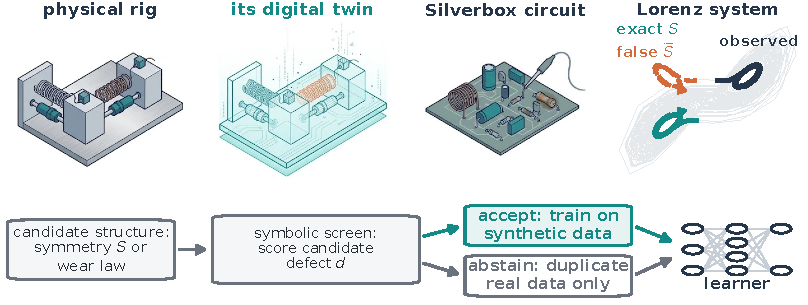
\includegraphics[width=0.88\linewidth]{figures/overview.pdf}
\caption{\textbf{Propose structure, test it, then train.} Candidate symmetries or wear laws arise from geometry or physics. Exact and false Lorenz reflections both reach the unseen wing but assert different dynamics. A symbolic fit scores each candidate by its defect $d$; accepted structure supplies training data, otherwise the learner uses duplication. Rig, twin and circuit are AI-generated illustrations; Lorenz trajectories are simulated.}
\label{fig:hero}
\end{figure}

Three questions matter. \textbf{(A)~Provenance:} what does a synthetic trajectory know beyond the observations that built its generator? \textbf{(B)~Learner response:} does its update improve deployment prediction? \textbf{(C)~Certifiability:} can its structural claim be checked without observing the deployment region? These answers can disagree. Self-labelled ridge rows do not move their own fit, yet can make its uncertainty spuriously small; wrong dynamics can rescue a poorly identified learner; and a verifier may accept structure where that structure is least useful to the verifier. A reliable twin therefore needs provenance, a learner-relative value test, and an explicit reason to trust its physics (Table~\ref{tab:regimes}).

\paragraph{Contributions.}
Information closure (Proposition~\ref{thm:closure}) is our baseline, not a new data-processing theorem. The contributions are its operational consequences. \textbf{(A)~Misleading confidence:} an exact law predicts how counting synthetic labels as independent degrades interval coverage (Proposition~\ref{prop:overconf}). \textbf{(B)~Learner-relative utility:} a block update and deployment-weighted theorem explain why wrong dynamics can help and why biased generators may have an interior optimal exposure (Theorem~\ref{thm:excitation}). \textbf{(C)~Limits of trust:} we bound symmetry defects by the verifier's unseen-region error, derive a conditional finite-sample certificate, and measure the cost of abstention (Proposition~\ref{prop:sandwich}; Theorem~\ref{thm:selective}). We test Lorenz, Duffing, four real benchmarks, and a maintenance twin.

\paragraph{Related work.}
\emph{Experiment design} chooses informative inputs, from persistent excitation to application-oriented design \citep{ljung1999system,hjalmarsson2005experiment,gevers2005identification,bombois2006least,rojas2007robust,huan2024oed}; our excitation result instead studies a possibly biased synthetic source. \emph{Synthetic rollouts} face compounding error in Dyna and MBPO \citep{sutton1990dyna,janner2019mbpo}, while self-consuming loops can degrade \citep{shumailov2024collapse,alemohammad2024mad,dohmatob2024regression}. Work on LLM synthesis asks what closed loops can add \citep{li2026information,dale2026synthetic}. Recent L4DC methods filter world-model data, correct simulators, learn constitutive laws, or select data for control \citep{kim2026wombet,lanier2026redraw,patkar2026bgcl,naf2026choose}; here we ask what synthetic data contain, how they move a learner, and what can be checked first. \emph{Structure} is proposed or exploited through symbolic identification, symmetry discovery, constrained models and invariant augmentation \citep{brunton2016sindy,yang2023liegan,yang2024symmetry,calvobarles2025equivariance,tahmasebi2026adaptive,wang2021symmetry,valperga2022reversible,dao2019kernel,chen2020group,ordonez2023discrete,wang2022data,brandstetter2022lie}. We instead test certification from one-sided data and transfer to a separate learner. Predictive maintenance motivates this setting \citep{nieminen2026synthetic,wuttke2026digital}; trusted physics can also be incorporated directly through Bayesian twin updating \citep{kapteyn2021probabilistic} (Supplement~\ref{app:bayes-twins}).

\section{Provenance and learner response (A, B)}\label{sec:theory}
Convert a trajectory into design-response rows $(\Phi,Y)$ and fit
\begin{equation}\label{eq:ridge}
\hTh=(\Phi^\top\Phi+\lambda I)^{-1}\Phi^\top Y,\qquad H:=\Phi^\top\Phi+\lambda I\succ0.
\end{equation}
An added trajectory contributes $(C,U)$; let $H_C=H+C^\top C$ and $R_C=U-C\hTh$.

\begin{lemma}[Exact finite-block update]\label{lem:update}
\begin{equation}\label{eq:update}
\Delta_C:=\hTh_C-\hTh=H_C^{-1}C^\top R_C.
\end{equation}
\end{lemma}
\ProofSketch Subtract the base and augmented normal equations and left-multiply by $H_C^{-1}$. \hfill$\square$
\begin{corollary}[Self-consistency limit]\label{cor:self}
If the generator uses the same fitted map and representation, $U=C\hTh$, then $R_C=0$ and $\Delta_C=0$ exactly.
\end{corollary}
\Intuition A self-labelled rollout may visit new states, but for this learner its labels contain no disagreement capable of moving the estimator.

\begin{proposition}[Information closure: the model-agnostic statement]\label{thm:closure}
Let the physical parameter be $\theta$, $D\sim p_\theta$, and let synthetic trajectories be sampled from a Markov kernel $K(\mathrm dz\mid D)$ with no access to $\theta$ except through $D$. Then
\begin{equation}\label{eq:closure}
p_\theta(D,Z)=p_\theta(D)K(Z\mid D),\qquad \mathcal I_{D,Z}(\theta)=\mathcal I_D(\theta).
\end{equation}
In a Bayesian model, $p(\theta\mid D,Z)=p(\theta\mid D)$ and $I(\theta;Z\mid D)=0$.
\end{proposition}
\ProofSketch Conditional on $D$, the kernel is $\theta$-independent. Hence the joint score is exactly the score of $D$; Bayes' rule gives the posterior identity. \hfill$\square$
\Intuition This is standard data processing, not our novelty claim. It distinguishes the \emph{source} of information from the \emph{format} used to deliver it: an external law can be encoded as training rows, whereas a data-only generator cannot create a new physical measurement. Neither statement determines a learner's risk or validates the law; a different learner can change its predictions when it consumes self-generated rows without gaining new physical evidence. Those are the questions addressed next (Supplement~\ref{app:closure-proof}).

For $U=C\Theta_g+E_g$, define $W_r=H_C^{-1}H$ and $W_s=H_C^{-1}C^\top C$. Then
\begin{equation}\label{eq:pull}
\hTh_C=W_r\hTh+W_s\Theta_g+H_C^{-1}C^\top E_g,\qquad W_r+W_s=I.
\end{equation}
This is the competition between learner and generator. Its high-probability form (Proposition~\ref{prop:finite}, Supplement~\ref{app:finite}) shows that, for an equation-error design, the twin enters only through added excitation and its own mismatch $\|C(\theta_g-\theta_\star)\|$, which vanishes for a correct twin.

\subsection{Deployment-weighted synthetic value}
Equal-size duplication is the baseline because regularization and exposure can move a fit even without new content. For validation residual $R_v=Y_v-\Phi_v\hTh$, candidate/duplicate updates $\Delta_a,\Delta_s$ obey
\begin{equation}\label{eq:value}
V=\frac{2}{N_v}\ip{\Phi_v^\top R_v}{\Delta_a-\Delta_s}_F+
\frac{\norm{\Phi_v\Delta_s}_F^2-\norm{\Phi_v\Delta_a}_F^2}{N_v}.
\end{equation}
Thus value depends on alignment with unresolved deployment error, not movement alone.

\begin{theorem}[Deployment-weighted synthetic excitation]\label{thm:excitation}
Vectorize the parameter and let $e=\widehat\theta-\theta_\star$, $g=\theta_g-\theta_\star$, and $\mathcal R_Q(e)=e^\top Qe$, $Q\succeq0$. Add noiseless synthetic information $G=\rho vv^\top$ from generator $\theta_g$. Define
\[
h=v^\top H^{-1}v,\quad s=v^\top(e-g),\quad m=v^\top H^{-1}Qe,\quad c=v^\top H^{-1}QH^{-1}v.
\]
With $\alpha=\rho/(1+\rho h)$,
\begin{equation}\label{eq:rankone-risk}
e_\rho=e-\alpha H^{-1}vs,\qquad
\mathcal R_Q(e_\rho)-\mathcal R_Q(e)=-2\alpha sm+\alpha^2s^2c.
\end{equation}
Hence $sm\le0$ cannot benefit from positive exposure; for $s\ne0,c>0$, the best effective exposure is the projection of $m/(sc)$ onto $[0,h^{-1}]$, so a biased source can have a finite optimum and excessive exposure can become harmful. For a small matrix budget $G=tA$, $A\succeq0$, $\tr A\le\tau$, writing $a=H^{-1}Qe$ and $b=e-g$ gives
\begin{equation}\label{eq:optimal-direction}
-\left.\frac{d}{dt}\mathcal R_Q(e_t)\right|_0=2\tr[A\operatorname{Sym}(ab^\top)],
\end{equation}
so the best nonzero infinitesimal design is rank one along the top eigendirection of $\operatorname{Sym}(ab^\top)$; otherwise $A=0$ is optimal.
\end{theorem}
\ProofSketch Sherman--Morrison gives $e_\rho$; substitute into $e^\top Qe$. Differentiating $(H+tA)^{-1}(He+tAg)$ gives \eqref{eq:optimal-direction}; linear optimization over $A\succeq0$, $\tr A\le\tau$ concentrates mass on the top eigendirection. \hfill$\square$
\Intuition Synthetic data help only when three things agree: the data excite a learnable direction, the generator's update points toward the deployment error there (it can help while less accurate than the learner), and deployment cares about that direction (Supplement~\ref{app:excitation-proof}). The first-order benefit $2\alpha sm$ equals, in expectation, the first term of \eqref{eq:value} on deployment-region validation data, which a practitioner can compute; without such data the theorem explains rather than decides (Section~\ref{sec:limits}). With noisy regressors it holds about the attenuated target, so a correct noiseless twin is a biased source for a model fed raw sensors (Corollary~\ref{cor:eiv}).

\begin{proposition}[No feature-only utility certificate]\label{prop:leverage}
Fix $H$ and candidate features $C$. Any statistic $T(C,H)$ is identical for every choice of synthetic targets $U$, yet two target blocks on the same $C$ can induce opposite deployment-risk changes. Hence no feature-only score can determine the sign of synthetic utility in general.
\end{proposition}
\ProofSketch Vary $U$ with $(C,H)$ fixed; see Supplement~\ref{app:feature-proxy}. \hfill$\square$
\Intuition Leverage sees \emph{where rows land} ($h$), not whether their labels point the right way ($s,m,c$).

\section{Learner response in controlled dynamics (B)}\label{sec:experiments}
We use Lorenz-63, equivariant under $S(x,y,z)=(-x,-y,z)$, and conservative Duffing $\ddot x=x-x^3$, equivariant under $S(x,\dot x)=(-x,-\dot x)$. Training sees one Lorenz wing or one Duffing well. Every augmentation is matched by equal-length duplication.

\paragraph{Protocol.} Learners are AR(4) models and polynomial increment libraries (degree 2 for Lorenz, 3 for Duffing), with ridge regularization tuned per arm. A seed is eligible when genuine missing-region data improve calibration error over duplication, which removes seeds where no data could help and changes no sign (all-seed results: Supplement~\ref{app:results}). Arms: \emph{own-model rollout} (the learner's own labels), \emph{exact}/\emph{false reflection} (mirrored real data under the true/a wrong symmetry), \emph{missing-region real} (genuine unseen-wing data, an oracle), \emph{simulator}.

\begin{table}[t]
\centering\small
\caption{Duplicate-adjusted gains in recursive balanced-test NRMSE ($h\in\{1,4,8\}$, eligible seeds; positive is better; non-rollout entries have 95\% intervals excluding zero, Supplement~\ref{app:results}). Last row: base error on the unseen over the observed region, an oracle whose label-free counterpart is the gate defect (Section~\ref{sec:neurosym}).}
\label{tab:keyarms}
\setlength{\tabcolsep}{4.2pt}
\begin{tabular}{lrrrr}
\toprule
Arm & Lorenz AR(4) & Lorenz quadratic & Duffing AR(4) & Duffing cubic\\
\midrule
Own-model rollout & $-0.000$ & $+0.004$ & $+0.000$ & $+0.121$\\
False reflection & $+0.028$ & $\mathbf{-0.061}$ & $+0.090$ & $+1.368$\\
Exact symmetry & $+0.066$ & $+0.055$ & $+0.107$ & $+1.469$\\
Missing-region real & $+0.063$ & $+0.056$ & $+0.109$ & $+1.470$\\
Simulator & $+0.062$ & $+0.057$ & $+0.109$ & $+1.468$\\
\midrule
Unseen\,/\,observed error & $2.9\times$ & $1.3\times$ & $2.1\times$ & $23\times$\\
\bottomrule
\end{tabular}
\end{table}

\begin{figure}[t]
\centering
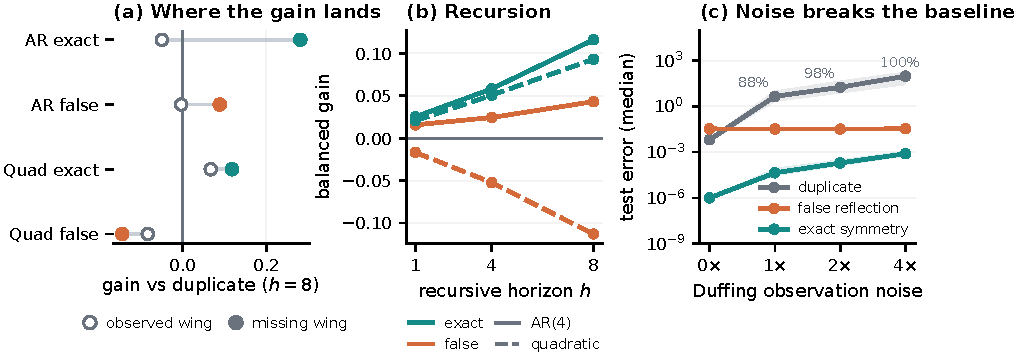
\includegraphics[width=0.80\linewidth]{figures/synthetic_comparisons.pdf}
\caption{\textbf{Support alone does not determine value.} (a) False reflection helps the AR learner but harms the quadratic library on the unseen wing. (b) Recursion amplifies this contrast. (c) Noise sweep (40 seeds per level; interquartile bands): the false reflection rescues a deteriorating duplicate-only fit without becoming physically correct. Labels count seeds with error $>1$.}
\label{fig:empirical}
\end{figure}

Own-model rollouts are inert for the AR learners (Corollary~\ref{cor:self}); exact symmetry matches genuine missing-region data and a simulator everywhere (Table~\ref{tab:keyarms}). The false reflection helps the Lorenz AR ($+0.028$) and both Duffing learners but harms the quadratic library ($-0.061$). The last row explains why: that library already forecasts the unseen wing almost as well as the seen one ($1.3\times$), so a wrong source can only pull it away (in Theorem~\ref{thm:excitation}'s terms, $sm>0$ only where the source pulls toward the deployment truth). When a learner extrapolates badly ($2$--$23\times$), reaching the missing region matters most and correctness adds a smaller margin.

Holding the one-well coverage construction fixed while changing observation noise (Fig.~\ref{fig:empirical}c) reverses Duffing's verdict: the false reflection harms all 40 noise-free learners but helps all 40 at nominal noise, when duplicate-only training deteriorates. This supports a learner-identification explanation, without isolating one unique noise mechanism. Feature novelty cannot resolve the verdict: exact and false blocks have similar leverage, yet the false one helps 0/40 Lorenz and 40/40 Duffing seeds in the corresponding one-step study (Supplement~\ref{app:interventions}; Proposition~\ref{prop:leverage}).

\section{Certifying structure before use (C)}\label{sec:neurosym}
\textbf{Geometry is the interface:} candidate transformations act on state space, a symbolic model scores them, and only accepted structure becomes data for the separate learner. Fit a symbolic field $\widehat f_\theta(x)=F(x)\widehat\theta$ to the observed data and score each candidate orthogonal $S$ (here all nonidentity axis sign flips) by
\begin{equation}\label{eq:defect}
d(S)=\frac{\left(\frac1n\sum_i\|\widehat f_\theta(Sx_i)-S\widehat f_\theta(x_i)\|_2^2\right)^{1/2}}
{\left(\frac1n\sum_i\|\widehat f_\theta(x_i)\|_2^2\right)^{1/2}}.
\end{equation}
The gate says yes only when the best candidate fits the seen data well ($d_{(1)}\le0.5$) and has at most half the defect of the runner-up ($d_{(1)}/d_{(2)}\le0.5$); otherwise it abstains and the learner falls back to duplication.

No such test can be uniformly safe and powerful: a smooth bump where no data were seen breaks the symmetry without changing an observation (Supplements~\ref{app:symmetry},~\ref{app:screening-bound}). A low defect is informative only through the fitted field's accuracy on reflected states. Write $E=\widehat f-f$ for the error of the symbolic fit and $e_X=\|E\|_{X,2}$, $e_{SX}=\|E\|_{SX,2}$ for its RMS size on the observed states and on their mirror images (all divided by $\|\widehat f\|_{X,2}$, as in \eqref{eq:defect}).

\begin{proposition}[What the defect measures]\label{prop:sandwich}
Let $S$ be orthogonal. (a) \emph{Safety:} the physical field's defect satisfies $d_f(S)\le d(S)+e_{SX}+e_X$. (b) \emph{Certification is an extrapolation measurement:} if $S$ is a true symmetry, $f(Sx)=Sf(x)$, then
\begin{equation}\label{eq:sandwich}
|e_{SX}-e_X|\;\le\; d(S)\;\le\; e_{SX}+e_X .
\end{equation}
(c) \emph{Time reversal:} for a mechanical system $\dot x=v$, $\dot v=g(x)$ and $S(x,v)=(x,-v)$, $d_f(S)=2$ exactly.
\end{proposition}
\ProofSketch (a) and (b) insert $\widehat f(Sx_i)$ and $S\widehat f(x_i)$, use $\|S\|=1$ and the triangle and Minkowski inequalities; for (b), $f(Sx)-Sf(x)=0$ leaves $E(Sx)-SE(x)$. (c) $f(Sx)-Sf(x)=(-2v,2g(x))=-2f(x)$. Supplement~\ref{app:sandwich}. \hfill$\square$
\Intuition For a true symmetry the defect is not really a property of the symmetry at all: it measures how wrong the fitted model is on the mirror region it never saw, give or take its error on the data. So a small defect means a small unseen-region error only when the fit to the data ($e_X$) is also good. So the gate can only certify a symmetry when the verifying model already extrapolates well, which is when that symmetry has least left to teach that model; it is a conditional screen, not a guarantee of physical correctness. By (c), threshold $0.5$ passes Duffing's time reversal only if $e_{SX}+e_X\ge1.5$.

\begin{figure}[!tbp]
\centering
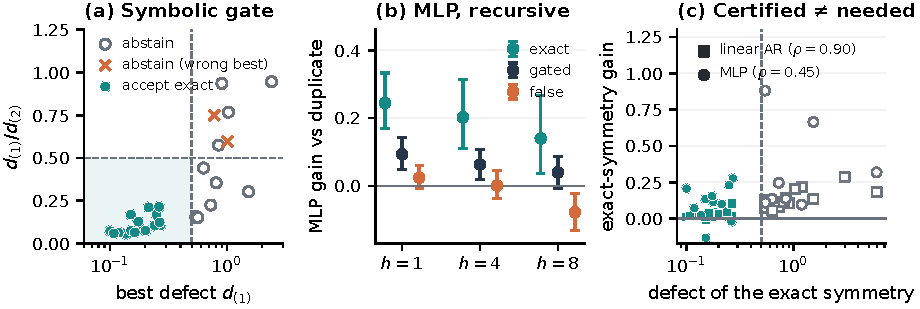
\includegraphics[width=0.68\linewidth]{figures/symmetry_verification.pdf}
\caption{\textbf{Lorenz: selective screening and neural payoff.} (a) On fresh seeds, the gate accepts the exact reflection 17/30 times, with no wrong acceptance; crosses mark incorrect lowest-defect candidates. (b) Recursive MLP gains (20 seeds; 95\% intervals). (c) Accepted seeds (filled) tend to have less exact-symmetry benefit for the verifier and, here, the MLP.}
\label{fig:neurosym}
\end{figure}

\paragraph{When the gate can certify.} On Lorenz the gate picks the correct reflection in 17 of 30 fresh seeds and never a wrong one (Fig.~\ref{fig:neurosym}a); on a symmetry-free Lotka--Volterra control it accepts nothing, while a ratio-only rule is fooled in 6 of 30. A sparse-library variant made one wrong accept (Supplement~\ref{app:reruns}). On noisy Duffing it abstains everywhere, as Proposition~\ref{prop:sandwich} predicts (Supplement Fig.~\ref{fig:duffing-neurosym}); without noise it certifies the exact symmetry in 29 of 30 seeds.


\paragraph{What the gate buys a neural learner.} Accepted transformations augment a separate MLP. On recursive forecasts (Fig.~\ref{fig:neurosym}b; 20 fresh seeds, 12 accepted, all exact), always-exact symmetry gains $+0.195$ $[0.110,0.301]$ over duplication and the gated arm gains $+0.065$ $[0.023,0.109]$, while the false reflection is no better than duplication (Supplements~\ref{app:reruns},~\ref{app:neuralfresh}).

\paragraph{Real data: the Silverbox circuit.} The Silverbox circuit \citep{wigren2013three} realizes $m\ddot y+d\dot y+(a+by^2)y=u$, whose idealized dynamics are odd under $(y,u)\mapsto(-y,-u)$; training keeps rows with $y_{t-1}>0$ (Supplement~\ref{app:silverbox}). A cubic NARX library gives the nominal candidate a defect of $0.002$ (false and input-only: $0.30$), so the gate accepts it in 10/10 records, and the defect equals the library's unseen-half error, as Proposition~\ref{prop:sandwich} predicts. Mirrored data then match genuine unseen-half data; the false reflection multiplies errors at least five-fold at $h=50$, not at every horizon. On a Wiener--Hammerstein record \citep{schoukens2009wh}, where the reflection is only approximate, the gate accepts it in four of five records (defect $0.31$--$0.41$) and the mirror cuts the cubic error by $87\%$ (Supplement~\ref{app:wh}).

\paragraph{Real data: a worn positioning drive.} On the EMPS ball-screw drive \citep{janot2019emps} the textbook friction law is odd, but screw fatigue makes viscous friction 44\% larger at negative velocity, so the mirror $(v,F)\mapsto(-v,-F)$ is only approximate (true defect $0.17$). From positive-velocity rows (Supplement~\ref{app:emps}) a generic cubic verifier abstains, while the textbook-law verifier accepts the mirror in 4/4. Mirrored rows then cut half-second error by 49--83\% across three learners (MLP improvement in 14/20 paired runs), yet stay three times above genuine data for two: the unseen asymmetry is the bound's mismatch term.

\paragraph{Certification is easiest where it is least needed.} With the true fields known, \eqref{eq:sandwich} holds on all 90 fresh seeds and the exact symmetry's defect tracks the fit's mirror-region error almost one-for-one (Spearman $0.99$--$1.00$). The defect is a label-free measurement of extrapolation error, which is what augmentation repairs; so it correlates positively with the exact symmetry's gain ($\rho=0.90$, $0.60$, $0.45$ for the Lorenz AR, library and MLP; Fig.~\ref{fig:neurosym}c), and gating recovers only 17--33\% of that gain: the gate is a safety diagnostic, not an accuracy method. This concerns the verifier's own class: a strong verifier can certify what a weaker learner needs (Silverbox).

\section{A predictive-maintenance digital twin (A--C)}\label{sec:digital-twin}
A two-DOF controlled asset obeys
\begin{equation}\label{eq:twin-mechanics}
M\ddot q+C(w)\dot q+K(w)q=Bu,
\end{equation}
where wear $w\in[0,1]$ lowers support stiffness and raises damping. A frozen 40-seed protocol trains a ridge learner at $w\le0.15$ and tests at $w\in\{0.55,0.70,0.85\}$ (Supplement~\ref{app:digital-twin}).


\begin{figure}[!tbp]
\centering
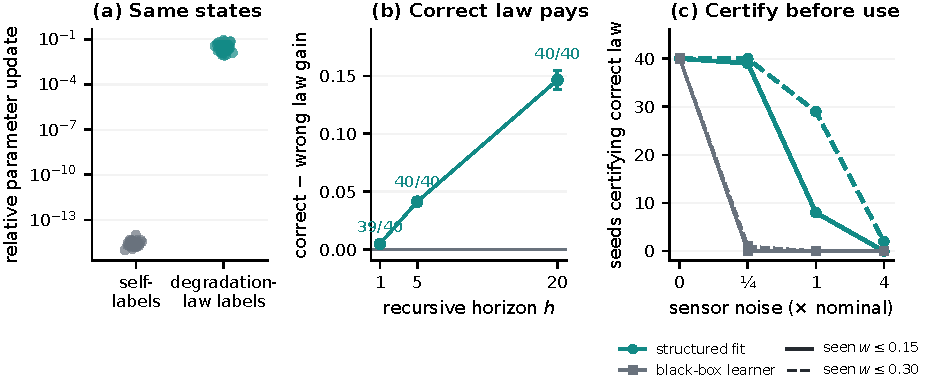
\includegraphics[width=0.72\linewidth]{figures/twin_experiments.pdf}
\caption{\textbf{Digital twin: identical states, different information.} (a) A degradation law changes the fitted learner; self-labels do not (Corollary~\ref{cor:self}). (b) Correct versus damping-only law (95\% intervals; wins out of 40). (c) The symbolic screen certifies more often than the black-box learner, but abstains with higher noise or narrower observed wear. No pairwise wrong acceptance (five-law screen: one in 480).}
\label{fig:digital-twin-results}
\end{figure}


Labelling the \emph{same} high-degradation states with the degradation law improves the median $h=20$ error by $0.762$, whereas self-labels give a floating-point-level update (Fig.~\ref{fig:digital-twin-results}a, Corollary~\ref{cor:self}). A learned twin gives $I(\theta;Z_{\rm self}\mid D)=0$; a degradation law \emph{transports} symbolic knowledge into data any learner can use (grey-box alternatives, at least as accurate where a learner exposes them: Supplement~\ref{app:greybox}).

The plausible wrong twin also helps ($sm>0$), but the correct one's paired advantage grows with horizon, from $0.005$ at $h=1$ to $0.147$ at $h=20$ (Fig.~\ref{fig:digital-twin-results}b), as the $H_f$-step risk $Q_{H_f}$ increasingly weights degradation-sensitive modes (Corollary~\ref{cor:horizon_geometry}).


\paragraph{Testing the exposure theorem.} Weighting a fixed block by $\rho$ reveals Theorem~\ref{thm:excitation}'s three regimes (Supplement Fig.~\ref{fig:exposure}): far from the truth every law helps and then saturates at its own bias; close to the truth the correct law peaks near $\rho=0.1$ in all 40 seeds and wrong laws end over 25 times above their best; when the learner is already right, any exposure hurts.

\paragraph{Certify the law before trusting the twin.} From light-wear data the gate, read off the twin's symbolic structure, prefers the correct law to the damping-only twin in 39/40 seeds at quarter noise and in 8/40 or 29/40 at nominal noise, never the wrong one (Fig.~\ref{fig:digital-twin-results}c; Supplement~\ref{app:twin-screen}).

\paragraph{Real data: cascaded tanks.} In this benchmark \citep{schoukens2017three,schoukens2016tanks}, a pump feeds two tanks with Bernoulli outflow $\sqrt x$ or, as a rival law, $x$. From levels $y\le6$\,V (two records; Supplement~\ref{app:tanks}) the gate abstains in both, since the square-root law's defect is only $1.2$--$1.8\times$ smaller; yet at high levels a square-root twin cuts an MLP's one-step error about six-fold and a linear one 1.5-fold, so abstaining forgoes a large gain.

\section{What cannot be certified, and a hidden cost (A, C)}\label{sec:limits}
\begin{figure}[t]
\centering
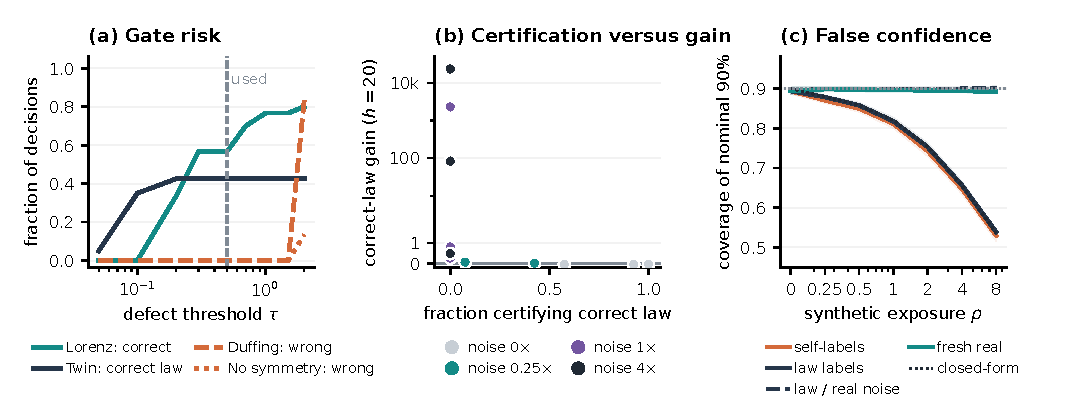
\includegraphics[width=0.98\linewidth]{figures/risk_and_coverage.pdf}
\caption{\textbf{Why selection and uncertainty need separate checks.} (a) Correct and wrong acceptances at representative thresholds (ratio fixed at $0.5$; 30--40 seeds; full sweep in Supplement~\ref{app:riskcov}). (b) Twin: certification rate versus correct-law gain across 12 wear--noise conditions (colours: noise). (c) Nominal 90\% coverage (medians, 40 seeds); dotted: Proposition~\ref{prop:overconf}(a).}
\label{fig:limits}
\end{figure}
\paragraph{What the gate risks.} In the 180 symmetry decisions, increasing the defect threshold from $0.5$ to $1.5$ raises Lorenz acceptances from 17 to 23/30 with no wrong acceptance; errors emerge at $2$ (Fig.~\ref{fig:limits}a; Supplement~\ref{app:riskcov}). The finite-sample bound (Theorem~\ref{thm:selective}) also depends on verifier leverage at reflected states and certifies nothing from one-sided data. The practical gate remains a screen. Pooled risk conceals a serious corner case: the twin's one wrong law is one of four acceptances in its setting, versus 1 in 167 overall.

\paragraph{Certified where least needed.} Across twelve twin settings (Fig.~\ref{fig:limits}b), certification is most frequent without noise, where the law slightly hurts ($h=20$: $-0.03$), and absent at nominal or greater noise, where the law rescues a diverging learner (gains $0.27$ to $>10^3$). This mirrors the symmetry result in Proposition~\ref{prop:sandwich}.

\paragraph{Counting synthetic rows as independent manufactures confidence.} This dependence problem is known; here we quantify its size and test remedies.
\begin{proposition}[Naive synthetic overconfidence]\label{prop:overconf}
Let $Y=\Phi\theta_\star+E$ with $E\sim\mathcal N(0,\sigma^2I_n)$ and $p$ parameters, and add $m$ self-labelled rows $(C,C\widehat\theta)$ with weight $\rho$. A pipeline that counts them as observations keeps $\widehat\theta$ (Corollary~\ref{cor:self}) but estimates $\widehat\sigma_\rho^2=k\,\widehat\sigma_0^2$ with $k=\frac{n-p}{n+\rho m-p}$, and its predictive interval at $x$ narrows by $\sqrt{k\,(1+\ell_\rho(x))/(1+\ell_0(x))}$, where $\ell_\rho(x)=x^\top(H+\rho C^\top C)^{-1}x$. (a) Where leverage is negligible, the coverage of a nominal $1-\alpha$ interval tends to $2\Phi(z_{\alpha/2}\sqrt k)-1$ as $n\to\infty$ with $\rho m/n$ fixed. (b) Estimating $\sigma^2$ from the real rows sets $k=1$ but keeps the leverage factor, which bites where $\ell_0(x)$ is large: in the unseen regime.
\end{proposition}
\ProofSketch Self-labels have zero residual, so the weighted residual sum is unchanged while the degrees of freedom grow by $\rho m$; the predictive variance is $\widehat\sigma^2(1+\ell(x))$, and $\widehat\sigma_0\to\sigma$ (Supplement~\ref{app:coverage}). \hfill$\square$
\Intuition Self-labels look like perfect measurements and falsely reduce estimated noise. The law predicts coverage within $0.011$ at every exposure (Fig.~\ref{fig:limits}c; $0.536$ predicted versus $0.530$ at $\rho=8$). Noiseless law labels behave similarly ($0.539$), whereas fresh real data retain $0.90$ coverage. Estimating noise from real rows repairs law-label coverage ($0.88$--$0.90$), but not self-labels in the unseen regime ($0.74$ versus $0.39$ naively).


\begin{table}[t]
\centering\small
\caption{What a twin user can claim and do, by the information available.}
\label{tab:regimes}
\begin{tabular}{@{}>{\raggedright\arraybackslash}p{0.24\linewidth}>{\raggedright\arraybackslash}p{0.72\linewidth}@{}}
\toprule
Information available & What can be claimed and done\\
\midrule
Deployment-regime real data & Estimate each block's duplicate-adjusted value \eqref{eq:value}, tune its exposure, estimate noise from real rows only.\\
A law or symmetry only & Screen candidates; read acceptance as conditional and abstention as a request for data; compare with duplication; impose the structure if the learner allows.\\
Neither & Self-generated trajectories are not evidence about unseen dynamics and must not shrink uncertainty; collect real data.\\
\bottomrule
\end{tabular}
\end{table}

\section{Discussion and conclusion}
The information-closure baseline is familiar; the operational lesson is not. A digital twin can be uninformative yet make its learner overconfident, physically incorrect yet improve deployment prediction, or structurally plausible yet impossible to certify from the observed regime. These outcomes are not contradictions: \emph{information provenance}, \emph{learner-relative value}, and \emph{verifier reliability} answer different questions. A small LQR check reduces closed-loop cost excess from $77\%$ to under $3\%$, but does not establish an advantage for the gate (Supplement~\ref{app:closedloop}).
\paragraph{Implication for digital-twin practice.} Record what knowledge each trajectory encodes; compare its downstream value against equal-size duplication, not only against no augmentation; calibrate uncertainty on independent real observations; and treat screening abstention as a request for coverage rather than proof that the physics is false. These are testable safeguards, not a guarantee that generated trajectories are useful or correct (Table~\ref{tab:regimes}). \textbf{Limitations:} ridge theory, sign-flip candidates, a simulated twin, and one device per real benchmark (Supplement~\ref{app:evaluation-profile}). \textbf{Code and archived data:} \url{https://github.com/pche123/l4dc-digital-twins}.


\paragraph{Generative AI Use.} Generative AI tools assisted ideation, derivations, coding, figures (including the illustrative renderings in Figure~\ref{fig:hero} and Supplement Figure~\ref{fig:emps-twin}), literature search and editing; the authors verified all AI-assisted content and take responsibility for the paper.

\acks{This work was supported by JST CREST Grant Number JPMJCR22D3, ``Machine Learning That Connects to Symbolic Reasoning.''}
\bibliography{refs}

\clearpage
\appendix
\makeatletter\def\presectionnum{Supplement~}\makeatother
\renewcommand{\theHfigure}{S\arabic{figure}}\renewcommand{\theHtable}{S\arabic{table}}\renewcommand{\theHequation}{S\arabic{equation}}
\section*{Supplementary Material}
\noindent\textbf{Reproduction guide.} Source code, archived experimental outputs, raw-data download guidance, and an itemized map from each main-paper figure/table to scripts and CSVs are at \url{https://github.com/pche123/l4dc-digital-twins} (see \texttt{docs/}). Historical raw-input reproduction is incomplete; the repository documents the boundary explicitly.\par\medskip
\noindent
The following supplementary material provides full derivations, protocol details,
additional recursive and neural results, symmetry-screening limits, digital-twin
diagnostics, reproducibility boundaries, and the broader Synthetic Information
Profile. The ten-page main paper appears before the references and this
contiguous supplement. The material below provides supporting proofs, experimental
details and additional results; the main scientific claims remain in the first ten pages.

\sloppy
\section{Proofs and algebraic details}\label{app:proofs}
Throughout, $\Phi\in\mathbb R^{n\times p}$, $Y\in\mathbb R^{n\times c}$, $\lambda>0$, $H=\Phi^\top\Phi+\lambda I\succ0$, and $\widehat\Theta=H^{-1}\Phi^\top Y$. An added block is $(C,U)$ with $C\in\mathbb R^{m\times p}$, $U\in\mathbb R^{m\times c}$, $H_C=H+C^\top C$, $R_C=U-C\widehat\Theta$, and $\Delta_C=\widehat\Theta_C-\widehat\Theta$.

\subsection{Information closure: posterior, Fisher information, and decision value}\label{app:closure-proof}
Let $D\sim p_\theta$ denote the authentic observations and let $Z\mid D\sim K(\cdot\mid D)$, where the synthetic kernel does not access $\theta$ except through $D$. Then
\[
p_\theta(D,Z)=p_\theta(D)K(Z\mid D).
\]
Under the usual differentiability and integrability conditions,
\[
\nabla_\theta\log p_\theta(D,Z)=\nabla_\theta\log p_\theta(D),
\]
so, whether Fisher information is defined as the score second moment or the negative expected Hessian,
\[
\mathcal I_{D,Z}(\theta)=\mathcal I_D(\theta).
\]
In a Bayesian formulation with prior $\pi(\theta)$,
\[
p(\theta\mid D,Z)=
\frac{\pi(\theta)p_\theta(D)K(Z\mid D)}{\int \pi(\vartheta)p_\vartheta(D)K(Z\mid D)d\vartheta}
=p(\theta\mid D),
\]
and hence $I(\theta;Z\mid D)=0$. Any Bayes action based on $(D,Z)$ can therefore be replaced by an action based on $D$ (plus the same independent randomization) with identical posterior risk. This is an information-sufficiency statement, not a claim that a restricted optimization algorithm cannot benefit from reparameterization, regularization, or additional compute. It also makes the provenance of useful synthetic information explicit: if external information $A$ enters and $Z\sim K(\cdot\mid D,A)$, then $I(\theta;Z\mid D,A)=0$; any physical information made available through $Z$ originates in $A$.

This is the system-identification specialization of the information-closed/data-processing viewpoint in \citet{li2026information}; related statistical work interprets synthetic augmentation as a way of injecting prior information rather than manufacturing observations \citep{dale2026synthetic}.

\paragraph{Why state a consequence of data processing?}
The posterior and Fisher identities are not claimed as new information theory. Their role is diagnostic: they separate \emph{epistemic information} from \emph{algorithmic value}. An information-closed block may still improve a restricted learner because it changes weights, regularization, optimization trajectory, representation geometry, or the approximation error of a misspecified model. Such a gain does not contradict $I(\theta;Z\mid D)=0$; it means the algorithm extracts the information already contained in $D$ differently. Conversely, when an external source $A$ enters, the loop is information-open relative to $D$ even though $Z$ adds no information conditional on $(D,A)$. This distinction is essential for interpreting pretrained generators, physics simulators, verifiers, or fresh environment interaction.

\subsection{Deployment-weighted synthetic excitation: full derivation}\label{app:excitation-proof}
For this subsection vectorize a single-output parameter, or equivalently apply the result to the vectorized multi-output problem with the corresponding block information matrix. Let the current and generator errors be
\[
e=\widehat\theta-\theta_\star,\qquad g=\theta_g-\theta_\star,
\]
and let deployment risk be $\mathcal R_Q(e)=e^\top Qe$ for $Q\succeq0$. A noiseless synthetic block with information matrix $G$ yields
\[
e_G=(H+G)^{-1}(He+Gg)
=e-(H+G)^{-1}G(e-g).
\]
For $G=\rho vv^\top$, Sherman--Morrison gives
\[
(H+\rho vv^\top)^{-1}\rho v
=\frac{\rho}{1+\rho v^\top H^{-1}v}H^{-1}v.
\]
\[
h=v^\top H^{-1}v,\quad s=v^\top(e-g),\quad
m=v^\top H^{-1}Qe,\quad c=v^\top H^{-1}QH^{-1}v,
\]
and $\alpha=\rho/(1+\rho h)$ therefore gives exactly
\[
e_\rho=e-\alpha H^{-1}vs.
\]
Expanding the deployment risk,
\[
\begin{aligned}
\mathcal R_Q(e_\rho)-\mathcal R_Q(e)
&=-2\alpha s\,e^\top QH^{-1}v
+\alpha^2s^2v^\top H^{-1}QH^{-1}v\\
&=-2\alpha sm+\alpha^2s^2c.
\end{aligned}
\]
If $c>0$, the quadratic is strictly convex in the effective exposure $\alpha$. Positive exposure improves on the base iff
\[
2sm>\alpha s^2c.
\]
Thus $sm\le0$ cannot help. When $sm>0$, improvement holds for
\[
0<\alpha<\frac{2m}{sc},
\]
and the unconstrained minimizer is $m/(sc)$. Because $\rho\in[0,\infty)$ maps monotonically to $\alpha\in[0,h^{-1})$, the optimal feasible effective exposure is
\[
\alpha_\star=\Pi_{[0,h^{-1}]}
\left(\frac{m}{sc}\right),
\]
with the boundary $h^{-1}$ interpreted as the $\rho\to\infty$ limit. If $0<\alpha_\star<h^{-1}$, the corresponding finite synthetic weight is
\[
\rho_\star=\frac{\alpha_\star}{1-\alpha_\star h}.
\]
This proves the first part of the deployment-weighted excitation theorem in the main paper and makes ``too much biased synthetic data'' mathematically precise.

For the small-budget matrix result, set $G=tA$, $A\succeq0$. Differentiating
\[
e_t=(H+tA)^{-1}(He+tAg)
\]
at $t=0$ gives
\[
\dot e_0=-H^{-1}A(e-g).
\]
Therefore, with $a=H^{-1}Qe$ and $b=e-g$,
\[
-\dot{\mathcal R}_Q(0)
=2e^\top QH^{-1}Ab
=2\tr\!\left[A\operatorname{Sym}(ab^\top)\right].
\]
Let $S=\operatorname{Sym}(ab^\top)$. Over the spectrahedron $A\succeq0$, $\tr A\le\tau$, linear optimization gives
\[
\max_A\tr(AS)=\tau[\lambda_{\max}(S)]_+,
\]
attained by $A^\star=\tau v_\star v_\star^\top$ for a top eigenvector whenever $\lambda_{\max}(S)>0$. Since $S$ has rank at most two, its two possible nonzero eigenvalues are
\[
\lambda_\pm=\frac{a^\top b\pm\|a\|\|b\|}{2}.
\]
Hence, unless $a$ and $b$ are antiparallel, the maximizing direction can be written
\[
v_\star\ \propto\ \frac{a}{\|a\|}+\frac{b}{\|b\|}.
\]
The optimal small-budget synthetic direction is therefore the bisector between the deployment-sensitive learner error $H^{-1}Qe$ and the generator advantage $e-g$.

\paragraph{Relation to optimal experimental design.}
Classical OED chooses where to collect real measurements, often to optimize Fisher-information or Bayesian decision criteria under a specified observation model. Here the added information matrix $A$ is paired with a potentially biased synthetic source through $b=e-g$, and the objective is the downstream deployment risk rather than identification precision alone. This changes the qualitative solution: $A=0$ can be optimal, and increasing exposure to a biased source can cross from benefit to harm. The result should therefore be read as a \emph{biased synthetic-design} calculation, not as a replacement for OED.

\paragraph{Exact multi-direction exposure (corollary).}
Let the synthetic information be $G=VRV^\top$ with $V\in\mathbb R^{p\times r}$ and $R\succ0$. Woodbury's identity gives $(H+G)^{-1}G=H^{-1}V(R^{-1}+V^\top H^{-1}V)^{-1}V^\top$, so with $h=V^\top H^{-1}V$, $s=V^\top(e-g)$, $m=V^\top H^{-1}Qe$, $c=V^\top H^{-1}QH^{-1}V$ and $K=(R^{-1}+h)^{-1}$,
\[
e_G=e-H^{-1}VKs,\qquad \mathcal R_Q(e_G)-\mathcal R_Q(e)=-2\,s^\top Km+s^\top KcKs .
\]
For $r=1$ this is \eqref{eq:rankone-risk} with $K=\alpha$. The identity is exact; \texttt{code/verify\_multidirection.py} reproduces it to relative error $10^{-11}$ over 2000 random instances ($p\le11$, $r\le5$). It shows that exposure directions interact only through $K$, so two directions that are individually beneficial can be harmful together when $s^\top KcKs$ outweighs $2s^\top Km$.

\paragraph{Noisy regressors (errors-in-variables).}
In identification from measured trajectories the regressors are themselves noisy. Suppose the real regressors are observed as $z=x+u$, where $u$ has mean zero and covariance $\Sigma_u$ and is independent of $x$ and of the output noise, and write $\Sigma_z=\Sigma_x+\Sigma_u$ for second moments.
\begin{corollary}[Synthetic excitation with noisy regressors]\label{cor:eiv}
A model deployed on raw measurements has excess risk $\mathcal R(\theta)=(\theta-\tilde\theta)^\top\Sigma_z(\theta-\tilde\theta)$ about the attenuated target $\tilde\theta=\Sigma_z^{-1}\Sigma_x\theta_\star$. Hence Theorem~\ref{thm:excitation} and the multi-direction identity hold exactly with $e=\widehat\theta-\tilde\theta$, $g=\theta_g-\tilde\theta$ and $Q=\Sigma_z$. In particular, provided $\Sigma_z\succ0$, a correct noiseless twin ($\theta_g=\theta_\star$) has $g=\Sigma_z^{-1}\Sigma_u\theta_\star$, which can be nonzero: it can therefore be biased for raw-sensor deployment and may have an interior best exposure beyond which additional synthetic data are harmful. Such an optimum requires the directional conditions of Theorem~\ref{thm:excitation}; bias alone does not imply it. For deployment on clean state estimates ($Q=\Sigma_x$, target $\theta_\star$), the same twin has $g=0$. A twin whose regressors carry matched noise $u'\sim u$ has population target $\tilde\theta$.
\end{corollary}
\begin{proof}
$\mathbb E[(z^\top\theta-y)^2]=\theta^\top\Sigma_z\theta-2\theta^\top\Sigma_x\theta_\star+\mathrm{const}$, because $\mathbb E[zy]=\mathbb E[(x+u)(x^\top\theta_\star+\varepsilon)]=\Sigma_x\theta_\star$; completing the square gives $\mathcal R$ with minimizer $\tilde\theta$. Theorem~\ref{thm:excitation} and the multi-direction identity are algebraic in $(H,e,g,Q)$ for any symmetric $Q\succeq0$ and any reference point, so they hold about $\tilde\theta$. Then $g=\theta_\star-\tilde\theta=\Sigma_z^{-1}(\Sigma_z-\Sigma_x)\theta_\star=\Sigma_z^{-1}\Sigma_u\theta_\star$. For the matched twin the population normal equations are $\mathbb E[(c+u')(c+u')^\top]\theta=\mathbb E[(c+u')c^\top]\theta_\star$, that is $\Sigma_z\theta=\Sigma_x\theta_\star$, whose solution is $\tilde\theta$.
\end{proof}
\textbf{Intuition:} a model that will be fed noisy sensors should not use the true physical parameters; it should shrink them, because part of every reading is noise. A twin simulated without sensor noise teaches the unshrunk physics, which is appropriate when deployment uses clean state estimates but can pull raw-sensor prediction away from its noise-attenuated target. Whether that pull ultimately hurts depends on the initial fit and the excited directions. The fix is to give the twin's rows the sensors' noise. Numerically (Table~\ref{tab:eiv}) the identity holds to relative error $2\times10^{-11}$ in 3200 cases; the correct noiseless twin has an interior optimum for raw-sensor deployment in every one of 400 problems and is harmful at high exposure in $99.8\%$ of them, while the same twin keeps improving clean-input deployment and the noise-matched twin stays well below the no-twin risk. On the noisy maintenance twin this gives a second possible reason, besides nominal parameter mismatch, for the correct law's interior optimum; we did not separate the two.
\begin{table}[t]\centering\small
\caption{Median deployment risk relative to no twin as the exposure of a twin block grows (400 random problems, $d=6$, \texttt{code/eiv\_check.py}).}\label{tab:eiv}
\begin{tabular}{@{}lcccccc@{}}
\toprule
Exposure $\rho$ & 0.03 & 0.1 & 0.3 & 1 & 3 & 30\\
\midrule
Correct noiseless twin, raw-sensor deployment & 0.925 & 0.832 & 0.871 & 1.732 & 3.459 & 5.459\\
Correct noiseless twin, clean-input deployment & 0.929 & 0.795 & 0.554 & 0.239 & 0.065 & 0.001\\
Noise-matched twin, raw-sensor deployment & 0.878 & 0.683 & 0.435 & 0.303 & 0.330 & 0.416\\
\bottomrule
\end{tabular}
\end{table}

\subsection{Dynamical horizon metric}\label{app:horizon-metric}
For $x_{k+1}=f_\theta(x_k,u_k)$ and initial state independent of $\theta$, define $J_k=\partial x_k/\partial\theta$ at $\theta_\star$. Chain rule gives
\[
J_0=0,\qquad J_{k+1}=A_kJ_k+B_k,
\quad A_k=\partial_xf_{\theta_\star}(x_k,u_k),\quad B_k=\partial_\theta f_{\theta_\star}(x_k,u_k).
\]
For a perturbation $e$,
\[
x_k(\theta_\star+e)-x_k(\theta_\star)=J_ke+O(\|e\|^2).
\]
Thus a weighted horizon loss satisfies
\[
\begin{aligned}
\sum_{k=1}^{H_f}\|x_k(\theta_\star+e)-x_k(\theta_\star)\|_{W_k}^2
&=\sum_{k=1}^{H_f}e^\top J_k^\top W_kJ_ke+O(\|e\|^3)\\
&=e^\top Q_{H_f}e+O(\|e\|^3),
\end{aligned}
\]
where $Q_{H_f}=\sum_kJ_k^\top W_kJ_k$. Substitution into the deployment-weighted excitation theorem in the main paper yields the horizon-sensitive optimal excitation direction in the horizon-sensitive excitation corollary in the main paper. This is a local statement: for large parameter errors or trajectories near bifurcations, higher-order terms can dominate.


\subsection{Local nonlinear deployment risk and relinearization}\label{app:nonlinear-risk}
\begin{corollary}[Horizon-sensitive excitation]\label{cor:horizon_geometry}
For $x_{k+1}=f_\theta(x_k,u_k)$, let $J_0=0$ and $J_{k+1}=A_kJ_k+B_k$, with $A_k=\partial_x f_{\theta_\star}$ and $B_k=\partial_\theta f_{\theta_\star}$. A local $H_f$-step rollout loss has
\begin{equation}\label{eq:horizon-Q}
\mathcal L_{H_f}(\theta_\star+e)=e^\top Q_{H_f}e+O(\|e\|^3),\qquad Q_{H_f}=\sum_{k=1}^{H_f}J_k^\top W_kJ_k.
\end{equation}
\end{corollary}
\Intuition For chaotic dynamics a longer horizon makes parameter error matter more but shrinks the region where this quadratic picture holds, so the exposure optimum of Theorem~\ref{thm:excitation} is a local guide, recomputed after material parameter moves (Supplement~\ref{app:nonlinear-risk}).

The quadratic metric $Q_{H_f}$ is exact only for the local second-order surrogate. Let $\mathcal L(\theta)$ denote the actual rollout loss and assume $\nabla \mathcal L(\theta_\star)=0$, $\nabla^2\mathcal L(\theta_\star)=2Q_{H_f}$, and
\[
\|\nabla^2\mathcal L(\theta_1)-\nabla^2\mathcal L(\theta_2)\|_{\mathrm{op}}
\le L_3\|\theta_1-\theta_2\|_2
\]
on the segment of interest. Taylor's theorem with integral remainder gives
\[
\mathcal L(\theta_\star+e)-\mathcal L(\theta_\star)
=e^\top Q_{H_f}e+R_3(e),
\]
with
\[
|R_3(e)|\le \frac{L_3}{6}\|e\|_2^3.
\]
To see the constant, write
\[
R_3(e)=\int_0^1(1-t)e^\top\{\nabla^2\mathcal L(\theta_\star+te)-\nabla^2\mathcal L(\theta_\star)\}e\,dt,
\]
and use the Lipschitz bound; $\int_0^1 t(1-t)dt=1/6$.

Consequently the closed-form exposure optimum from the deployment-weighted excitation theorem in the main paper is a global statement only for a fixed quadratic risk. For nonlinear dynamics it is a local design rule around the current linearization. A sequential implementation should use a trust region or recompute $J_k$ and $Q_{H_f}$ after a material parameter update:
\[
Q_{H_f}(\widehat\theta_0)\to \Delta_0\to \widehat\theta_1
\to Q_{H_f}(\widehat\theta_1)\to\cdots.
\]
For chaotic dynamics, products of state Jacobians can make both $Q_{H_f}$ and the higher-order constant grow rapidly with horizon, so the local validity radius may shrink even as long-horizon deployment becomes more sensitive to parameter error. This is precisely why the main text treats the dose-response optimum as a local prediction rather than a global guarantee.

\subsection{Quantitative precision--coverage limit for symmetry screening}\label{app:screening-bound}
The one-sided observation theorem later constructs a symmetric field and a nonsymmetric alternative with indistinguishable observations. More generally, let $P_0$ and $P_1$ be the observed-data laws under a true symmetry and a false-symmetry alternative, and let $A$ be the event that a screening rule accepts symmetry. Total variation implies
\[
P_0(A)\le P_1(A)+\operatorname{TV}(P_0,P_1).
\]
Therefore any rule satisfying the wrong-accept constraint $P_1(A)\le\delta$ must obey
\[
P_0(A)\le\delta+\operatorname{TV}(P_0,P_1)
\le\delta+\sqrt{\tfrac12D_{\mathrm{KL}}(P_0\|P_1)},
\]
where the second inequality is Pinsker. In the exact one-sided construction $P_0=P_1$, so power is at most $\delta$: uniformly safe acceptance necessarily has equally low coverage on that indistinguishable pair. This is the decision-theoretic form of the abstention barrier observed empirically on Duffing.

\subsection{Exact block update and generator pull}
The augmented normal equations are
\[
H_C\widehat\Theta_C=\Phi^\top Y+C^\top U=H\widehat\Theta+C^\top U.
\]
Also $H_C\widehat\Theta=H\widehat\Theta+C^\top C\widehat\Theta$. Subtraction gives
\[
H_C(\widehat\Theta_C-\widehat\Theta)=C^\top(U-C\widehat\Theta)=C^\top R_C,
\]
which proves the finite-block update lemma in the main paper. If $U=C\Theta_g+E_g$, substitute into the same normal equations to obtain the synthetic-pull identity in the main paper.

\subsection{A finite-sample bound for the augmented ridge learner}\label{app:finite}
The exact update is an identity; here is its high-probability form. Take one output column (for $k$ columns use $\delta/k$ in each). Let the real data be $Y=\Phi\theta_\star+E$, where $E_t$ is conditionally $\sigma$-sub-Gaussian given the past (the rows of $\Phi$ may depend on earlier noise, as in a trajectory), and let the synthetic block be $U=C\theta_g+E_g$ with $E_g$ conditionally $\sigma_g$-sub-Gaussian, where $E_g$ is simulation noise drawn after the twin is built, so that conditional on the real data $E_g$ is $\sigma_g$-sub-Gaussian and independent of $(C,\theta_g)$. The twin itself may be fitted on the real data: the identity below holds for any $\theta_g$, and only the mismatch term then becomes random, which the bound keeps as stated. A deterministic twin has $\sigma_g=0$. Write $G=C^\top C+\lambda I$ and $d$ for the parameter dimension.

\begin{proposition}[Finite-sample bound]\label{prop:finite}
Under these assumptions, with $G=C^\top C+\lambda I$ and probability at least $1-\delta$,
\[
\|\widehat\theta_C-\theta_\star\|_{H_C}\le\sigma\sqrt{\log\tfrac{\det H}{\lambda^{d}}+2\log\tfrac2\delta}+\sigma_g\sqrt{\log\tfrac{\det G}{\lambda^{d}}+2\log\tfrac2\delta}+\sqrt\lambda\|\theta_\star\|+\|C(\theta_g-\theta_\star)\|_2,
\]
and hence, by Cauchy--Schwarz, $|x^\top(\widehat\theta_C-\theta_\star)|\le\|x\|_{H_C^{-1}}$ times the right-hand side for every deployment feature $x$.
\end{proposition}
\textbf{Intuition:} the twin enters in exactly two places. It enlarges $H_C$, which shrinks $\|x\|_{H_C^{-1}}$ (the excitation benefit, largest where the real data left $x$ poorly known), and it adds a mismatch term that vanishes for a correct twin.
\begin{proof}
The normal equations give $H_C\widehat\theta_C=\Phi^\top Y+C^\top U$. Using $H\theta_\star=\Phi^\top\Phi\theta_\star+\lambda\theta_\star$ and $H_C\theta_\star=H\theta_\star+C^\top C\theta_\star$,
\[
H_C(\widehat\theta_C-\theta_\star)=\Phi^\top E+C^\top E_g+C^\top C(\theta_g-\theta_\star)-\lambda\theta_\star .
\]
Apply $H_C^{-1/2}$ and the triangle inequality. (a) Since $H_C\succeq\lambda I$, $\|H_C^{-1/2}\lambda\theta_\star\|\le\sqrt\lambda\|\theta_\star\|$. (b) Since $C^\top C\preceq H_C$, $\|H_C^{-1/2}C^\top\|_{\mathrm{op}}\le1$, so $\|H_C^{-1/2}C^\top C(\theta_g-\theta_\star)\|\le\|C(\theta_g-\theta_\star)\|$. (c) Since $H_C\succeq H$, $\|H_C^{-1/2}\Phi^\top E\|\le\|H^{-1/2}\Phi^\top E\|$, and by the self-normalized martingale bound of \citet{abbasiyadkori2011improved} this is at most $\sigma\sqrt{\log(\det H/\lambda^{d})+2\log(2/\delta)}$ with probability $1-\delta/2$. (d) Likewise $H_C\succeq G$ gives the twin-noise term, conditionally on the real data (so for the fixed design $C$), with probability $1-\delta/2$. A union bound completes the first claim. The second follows from Cauchy--Schwarz, $|x^\top v|\le\|x\|_{H_C^{-1}}\|v\|_{H_C}$.
\end{proof}
\paragraph{Mirrored rows (noise shared with the real data).} The gate's synthetic rows are the real rows transformed by an orthogonal $S$, so their noise is not independent of $E$. Let the real library be exact, $f=F\theta_\star$, with increments $y_i=f(x_i)+e_i$, and take $C=F(SX)$, $U=Sy$ (the mirrored states with mirrored increments, one output column at a time). Then $U-C\theta_\star=m+SE$ with $m:=Sf(X)-f(SX)$ the stacked symmetry violation, and the same algebra gives $H_C(\widehat\theta_C-\theta_\star)=\Phi^\top E+C^\top SE+C^\top m-\lambda\theta_\star$. The two noise terms are each a predictable design against sub-Gaussian noise, so each is bounded by the self-normalized inequality (at $\delta/2$ each, using $H_C\succeq H$ and $H_C\succeq G$), and $\|H_C^{-1/2}C^\top m\|\le\|m\|_2$. Hence with probability at least $1-\delta$,
\[
\|\widehat\theta_C-\theta_\star\|_{H_C}\le\sigma\sqrt{\log\tfrac{\det H}{\lambda^{d}}+2\log\tfrac2\delta}+\sigma\sqrt{\log\tfrac{\det G}{\lambda^{d}}+2\log\tfrac2\delta}+\sqrt\lambda\|\theta_\star\|+\|Sf(X)-f(SX)\|_2 .
\]
The mismatch term is exactly $\sqrt n\,\|f\|_{X,2}$ times the physical field's defect $d_f(S)$ of Proposition~\ref{prop:sandwich}, so it vanishes for a true symmetry and otherwise equals the amount by which $S$ breaks the physics. \textbf{Intuition:} mirrored data cost nothing in the bound when the mirror is a true symmetry (they only add excitation), and when it is not, the price is the size of the violation, which is what the gate's defect estimates from the seen data.

\paragraph{Numerical check and tightness.} The constants are conservative: in five simulated settings (correct and mismatched twins, noisy and noiseless, $d=6$ and $d=15$; \texttt{code/\allowbreak finite\_\allowbreak bound\_\allowbreak check.py}, 4000 draws each) in three mirrored-row settings (true, weakly and strongly broken symmetry, 3000 draws each) and for a misspecified twin fitted on the same data (noisy and deterministic, 4000 draws each) the bound was never violated and the realised error was a median $0.13$ to $0.87$ of it (closest when the mismatch term dominates), so we use it for its structure, not its numbers. The mismatch term cannot be improved in general: with no real data, noiseless synthetic rows and $\lambda\to0$, $\|H_C^{1/2}(\widehat\theta_C-\theta_\star)\|\to\|C(\theta_g-\theta_\star)\|$ exactly.

\paragraph{Scope: which dynamics the bound covers.} The self-normalized inequality needs each regressor row to be fixed before its noise is drawn (a predictable design) and the noise to be conditionally sub-Gaussian given the past. Equation-error models such as ARX, whose regressors are past outputs and inputs and whose noise enters only the current equation, satisfy this, so the bound applies to them as stated. It does not apply when the regressors are themselves measured with noise (output-error or errors-in-variables settings, such as noisy state measurements fed back as inputs), because the regressor noise is then correlated with the target noise; an errors-in-variables version would add a term of the order of that regressor noise. The recursive experiments include such observation noise, so for them the bound is a guide to the structure of the trade, not a guarantee. The exact exposure identity has no such restriction: Corollary~\ref{cor:eiv} restates it about the attenuated target that noisy regressors induce.

\subsection{Correct-data contraction in the training-information norm}
Let $W_r=H_C^{-1}H$. If $U=C\Theta_\star+E_g$ with $\mathbb E[E_g\mid\widehat\Theta,C]=0$, then
\[
\mathbb E[\widehat\Theta_C\mid\widehat\Theta,C]-\Theta_\star=W_r(\widehat\Theta-\Theta_\star).
\]
Moreover,
\[
H^{1/2}W_rH^{-1/2}=H^{1/2}(H+C^\top C)^{-1}H^{1/2}
=(I+H^{-1/2}C^\top C H^{-1/2})^{-1}.
\]
The matrix on the right is symmetric positive definite with eigenvalues in $(0,1]$. Therefore, for every matrix $D$,
\[
\|H^{1/2}W_rD\|_F\le \|H^{1/2}D\|_F,
\]
which proves the contraction inequality. This is a conditional-mean parameter statement; it is not a guarantee of lower realized finite-sample or multi-step deployment loss.

For a wrong generator, write $e=\widehat\Theta-\Theta_\star$ and $g=\Theta_g-\Theta_\star$. Then
\[
\mathbb E[\widehat\Theta_C]-\Theta_\star=W_re+W_sg,
\qquad W_s=H_C^{-1}C^\top C,
\]
and $W_r+W_s=I$. If $H$ and $C^\top C$ share an eigenvector $u$ with eigenvalues $\eta$ and $\gamma$, then along $u$ the new error is
\[
\frac{\eta}{\eta+\gamma}u^\top e+\frac{\gamma}{\eta+\gamma}u^\top g.
\]
Thus an incorrect source can improve a sufficiently poor existing fit in a direction it excites, but can also make an already-good fit worse.

\subsection{Duplicate-adjusted value and residual envelope}
For any update $\Delta$,
\[
N_vL_v(\widehat\Theta+\Delta)=\|R_v-\Phi_v\Delta\|_F^2
=\|R_v\|_F^2-2\langle\Phi_v^\top R_v,\Delta\rangle_F+\|\Phi_v\Delta\|_F^2.
\]
Taking the difference between duplicate update $\Delta_s$ and augmentation update $\Delta_a$ proves the duplicate-adjusted value identity in the main paper.

A useful corollary bounds the magnitude of duplicate-adjusted value. Let $\kappa_j=\|(H+C_j^\top C_j)^{-1}C_j^\top\|_2$ for $j\in\{a,s\}$ and
\[
M=\kappa_a\|R_a\|_F+\kappa_s\|R_s\|_F.
\]
Then the finite-block update lemma in the main paper gives $\|\Delta_j\|_F\le\kappa_j\|R_j\|_F$, hence
\[
|V|\le \frac{2}{N_v}\|\Phi_v^\top R_v\|_F M
+\frac{\|\Phi_v\|_2^2}{N_v}M^2.
\]
The second term follows from
\[
\left|\|\Phi_v\Delta_s\|_F^2-\|\Phi_v\Delta_a\|_F^2\right|
\le \|\Phi_v\|_2^2(\|\Delta_s\|_F+\|\Delta_a\|_F)\|\Delta_s-\Delta_a\|_F.
\]
The bound is deliberately conservative: near-zero learner-relative residual limits how much an arm can matter, but a large residual does not determine the sign of value.

\subsection{Woodbury form, feature-only impossibility, and target-blind leverage}\label{app:feature-proxy}
Using $K_C=CH^{-1}C^\top$,
\[
(H+C^\top C)H^{-1}C^\top(I+K_C)^{-1}=C^\top,
\]
so
\[
(H+C^\top C)^{-1}C^\top=H^{-1}C^\top(I+K_C)^{-1},
\]
which proves the Woodbury identity. If $k_i>0$ are the nonzero eigenvalues of $K_C$, then
\[
\ell(C)=\sum_i\frac{k_i}{1+k_i},
\]
so $0\le \ell(C)<\operatorname{rank}(C)$ for nonzero $C$. A scalar counterexample uses $H=C=1$, $\widehat\theta=1/2$, and deployment truth $0$: both $U=0$ and $U=2$ have identical $\ell=1/2$, while the refits are $1/4$ and $5/4$, respectively.


The example proves a more general impossibility. Let $T(C,H)$ be any deterministic statistic that uses only candidate features and the base information geometry. Holding $(C,H)$ fixed leaves $T$ unchanged while varying $U$ changes $R_C=U-C\widehat\Theta$ and therefore the update. The scalar pair above yields opposite changes in squared deployment error under the same value of every such $T$. Hence no feature-only score can determine the sign of downstream utility over unrestricted target assignments.

For the rank-one family in the deployment-weighted excitation theorem in the main paper, the missing quantities can be read explicitly:
\[
h=v^\top H^{-1}v\quad\text{(feature excitation)},
\]
\[
s=v^\top(e-g)\quad\text{(generator advantage relative to the learner)},
\]
\[
m=v^\top H^{-1}Qe\quad\text{(deployment alignment)},
\qquad
c=v^\top H^{-1}QH^{-1}v\quad\text{(deployment curvature)}.
\]
A leverage-like score can reflect $h$ but has no access to $s$ and no reason to encode $m$ or $c$. The null-space case makes the separation especially stark: if $QH^{-1}v=0$, then $m=c=0$ and
\[
\mathcal R_Q(e_\rho)-\mathcal R_Q(e)=0
\]
for every $\rho$, even though $h$ can be arbitrarily large. Conversely, the same feature direction can be helpful or harmful solely by changing $g$, hence $s$. The empirical Lorenz/Duffing leverage result is therefore an instance of a structural limitation of feature-only utility proxies, not merely a failure of one chosen statistic.

\subsection{Recursive-horizon sensitivity}
For square maps $A,B$ and $h\ge1$,
\[
A^h-B^h=\sum_{j=0}^{h-1}A^{h-1-j}(A-B)B^j.
\]
This telescopes directly. If $\|A^k\|_2\le M_A\gamma_A^k$ and $\|B^k\|_2\le M_B\gamma_B^k$ for $k<h$, then
\[
\|A^h-B^h\|_2\le M_AM_B\|A-B\|_2
\sum_{j=0}^{h-1}\gamma_A^{h-1-j}\gamma_B^j.
\]
A one-step ordering need not persist. For scalar truth $0.9$, estimates $1.0$ and $0.75$, and $x_0=1$, the first estimate is closer at one step but farther at horizon ten.

\subsection{Exact and false reflections as transformed vector fields}\label{app:conj}
If $x(t)$ solves $\dot x=f(x)$ and $S$ is invertible, then $w(t)=Sx(t)$ solves
\[
\dot w=f_S(w):=Sf(S^{-1}w).
\]
For Lorenz, $S_{\mathrm{true}}=\mathrm{diag}(-1,-1,1)$ satisfies $f_S=f$. For $S_{\mathrm{false}}=\mathrm{diag}(-1,1,1)$,
\[
f_S(x,y,z)=\big(-\sigma(x+y),\,-x(\rho-z)-y,\,-xy-\beta z\big),
\]
a different quadratic vector field. For conservative Duffing $f(x,v)=(v,x-x^3)$, the exact map $\mathrm{diag}(-1,-1)$ leaves $f$ invariant, while $\mathrm{diag}(-1,1)$ gives $f_S=-f$: the same energy contours traversed backwards.

\section{Protocol details}\label{app:protocol}
\paragraph{Lorenz recursive study.} Long simulations use RK4 with step $0.01$, a 3000-step burn-in, and 6000 retained states. Every split is drawn from an independent simulation. Wing windows contain at least 95\% of states on the required side; observation noise is added before transformations, and transformations are applied in raw coordinates before training-only standardization. The local AR uses four lagged states without intercept. The quadratic library uses all degree-$\le2$ monomials of the current standardized state and predicts the increment. For each arm and seed, ridge $\lambda\in\{10^{-6},\ldots,10\}$ is selected on tuning data. Eligibility requires genuine opposite-wing data to improve calibration error by at least 10\% over duplication.

\paragraph{Duffing recursive study.} The conservative oscillator $\ddot x=x-x^3$ uses RK4 step $0.1$. Windows start in one well with initial conditions restricted to energies below the barrier; a random burn-in randomizes phase. Windows contain 40 states with nominal observation noise $0.01$. The cubic library contains all monomials of $(x,\dot x)$ of degree at most three and predicts increments. Split logic, arm matching, tuning, eligibility, and metrics follow the Lorenz study.

\paragraph{Fresh neural reconstruction.} The standalone one-step neural reconstruction (Supplement~\ref{app:neuralfresh}) uses 20 new Lorenz seeds (12300--12319), independent simulations for training and each test side, eight positive-wing training windows and eight noise-free test windows per side, lag four, two hidden layers of 64 tanh units, full-batch Adam for 400 epochs, learning rate $0.003$, and weight decay $10^{-4}$. The polynomial symmetry screen uses the fixed selective thresholds $d_{(1)}\le0.5$ and $d_{(1)}/d_{(2)}\le0.5$. No thresholds or network settings were changed after inspecting these 20 outcomes. The recursive MLP study of the main text is a different one: two tanh layers of 32 units, seeds 1000--1019 (Supplement~\ref{app:reruns}).

\section{Additional recursive results}\label{app:results}
\begin{table}[H]
\centering\small
\caption{Table~\ref{tab:keyarms} without the eligibility filter: duplicate-adjusted recursive balanced-test gains ($h\in\{1,4,8\}$) averaged over all 30 seeds per system (the filter removed 4, 2, 0 and 0 seeds). Every sign is unchanged, and every non-rollout entry still has a 95\% interval excluding zero.}
\label{tab:allseed}
\setlength{\tabcolsep}{4.2pt}
\begin{tabular}{lrrrr}
\toprule
Arm & Lorenz AR(4) & Lorenz quadratic & Duffing AR(4) & Duffing cubic\\
\midrule
Own-model rollout & $-0.001$ & $+0.003$ & $+0.000$ & $+0.121$\\
False reflection & $+0.025$ & $-0.066$ & $+0.090$ & $+1.368$\\
Exact symmetry & $+0.060$ & $+0.049$ & $+0.107$ & $+1.469$\\
Missing-region real & $+0.056$ & $+0.051$ & $+0.109$ & $+1.470$\\
Simulator & $+0.058$ & $+0.052$ & $+0.109$ & $+1.468$\\
\bottomrule
\end{tabular}
\end{table}
\begin{table}[H]
\centering\small
\caption{Lorenz balanced-test error reduction relative to equal-length duplication (mean, 95\% interval).}
\begin{tabular}{lcc}
\toprule
Arm & Local linear AR(4) & Quadratic library\\
\midrule
Own-model rollout & $-0.000$ $[-0.002,0.001]$ & $+0.004$ $[-0.002,0.010]$\\
Other-model rollout & $+0.006$ $[0.002,0.011]$ & $-0.056$ $[-0.081,-0.032]$\\
Time warp & $-0.000$ $[-0.010,0.011]$ & $-0.033$ $[-0.056,-0.013]$\\
False reflection & $+0.028$ $[0.013,0.044]$ & $-0.061$ $[-0.092,-0.028]$\\
Same-wing real & $+0.027$ $[0.011,0.046]$ & $+0.053$ $[0.030,0.078]$\\
Exact symmetry & $+0.066$ $[0.042,0.096]$ & $+0.055$ $[0.036,0.077]$\\
Opposite-wing real & $+0.063$ $[0.041,0.089]$ & $+0.056$ $[0.040,0.073]$\\
Simulator & $+0.062$ $[0.040,0.090]$ & $+0.057$ $[0.038,0.079]$\\
\bottomrule
\end{tabular}
\end{table}

\begin{table}[H]
\centering\small
\caption{Duffing balanced-test error reduction relative to equal-length duplication (30 eligible seeds per learner; mean, 95\% interval).}
\begin{tabular}{lcc}
\toprule
Arm & Local linear AR(4) & Cubic library\\
\midrule
Own-model rollout & $+0.000$ $[-0.005,0.005]$ & $+0.121$ $[0.016,0.243]$\\
Other-model rollout & $+0.012$ $[0.009,0.016]$ & $+0.116$ $[-0.223,0.481]$\\
Time warp & $+0.004$ $[0.003,0.006]$ & $+0.135$ $[0.045,0.259]$\\
False reflection & $+0.090$ $[0.063,0.119]$ & $+1.368$ $[0.861,1.936]$\\
Same-well real & $+0.027$ $[0.004,0.055]$ & $+0.911$ $[0.457,1.421]$\\
Exact symmetry & $+0.107$ $[0.080,0.138]$ & $+1.469$ $[0.947,2.032]$\\
Opposite-well real & $+0.109$ $[0.082,0.139]$ & $+1.470$ $[0.963,2.033]$\\
Simulator & $+0.109$ $[0.082,0.138]$ & $+1.468$ $[0.955,2.038]$\\
\bottomrule
\end{tabular}
\end{table}

\section{Independent neural reconstruction}\label{app:neuralfresh}
\begin{table}[h]
\centering\small
\caption{Fresh 20-seed Lorenz neural reconstruction: balanced one-step standardized-MSE gain relative to duplication. Intervals are paired seed bootstraps.}
\begin{tabular}{lccc}
\toprule
Arm & Mean gain & 95\% interval & Seeds improved\\
\midrule
False reflection & $0.398$ & $[0.341,0.454]$ & $20/20$\\
Selective gate & $0.401$ & $[0.267,0.531]$ & $14/20$\\
Exact symmetry & $0.568$ & $[0.491,0.642]$ & $20/20$\\
\bottomrule
\end{tabular}
\end{table}
The selective gate accepts 14/20 seeds and every accepted transformation is $(-x,-y,z)$. In the six abstaining seeds the selective arm is exactly the duplicate by design. The paired exact-minus-false improvement is $0.170$ with 95\% bootstrap interval $[0.136,0.207]$. These results come from the standalone reconstruction whose seed-level outputs are in \texttt{data/\allowbreak lorenz\_\allowbreak documented\_\allowbreak protocol\_\allowbreak results.csv}. Its design differs from the original-protocol MLP of Supplement~\ref{app:reruns} in architecture (64 versus 32 hidden units), data (eight versus two training windows), optimiser and metric (one-step standardized MSE versus recursive NRMSE). The two studies agree that exact symmetry dominates and that the gate never accepts a wrong candidate. They disagree on the false reflection, which is worth 70\% of the exact gain here and nothing on recursive forecasts in the original-protocol study. The original-protocol MLP's $h=1$ column (Table~\ref{tab:mlp-recursive}) shows the false reflection is weak there even one step ahead, so the disagreement reflects the learner and data regime rather than the metric alone.

\section{Symmetry screening: what can and cannot be inferred}\label{app:symmetry}
\begin{figure}[h]
\centering
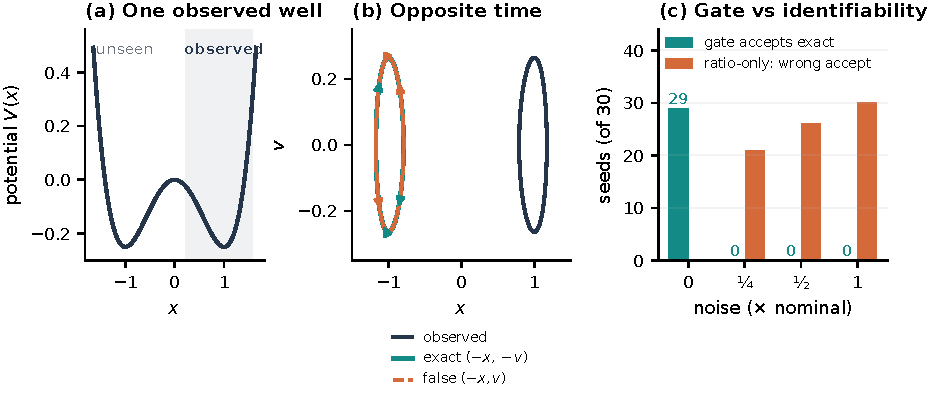
\includegraphics[width=\linewidth]{figures/duffing_dynamics.pdf}
\caption{\textbf{Duffing: same geometry, opposite time.} (a) Training observes one well. (b) The exact reflection $(-x,-v)$ and the false reflection $(-x,v)$ trace the same missing orbit with opposite orientation. (c) Fresh seeds per noise level: the gate certifies the exact symmetry only when the cubic library is identifiable (noise $0$) and never accepts a wrong candidate; a ratio-only rule accepts the time reversal whenever there is noise.}
\label{fig:duffing-neurosym}
\end{figure}

Define $\|g\|_{X,2}=(n^{-1}\sum_i\|g(x_i)\|_2^2)^{1/2}$ and $D_{\widehat f}(S;X)=\|\widehat f\circ S-S\widehat f\|_{X,2}$.

\begin{proposition}[Defect-transfer inequality]
For orthogonal $S$,
\[
D_f(S;X)\le D_{\widehat f}(S;X)+\|f-\widehat f\|_{SX,2}+\|f-\widehat f\|_{X,2}.
\]
\end{proposition}
\begin{proof}
For each $x_i$, insert and subtract $\widehat f(Sx_i)$ and $S\widehat f(x_i)$ inside $f(Sx_i)-Sf(x_i)$, apply the triangle inequality pointwise, then Minkowski across $i$ and $\|S\|_2=1$.
\end{proof}
This isolates the central extrapolation issue: a tiny learned defect on observed states says little if $\widehat f$ is inaccurate on reflected states $SX$.

\paragraph{Intuition:} the true field's asymmetry can hide only inside the fitted model's errors, on the data or on their mirror images.

\subsection{Proof of Proposition~\ref{prop:sandwich}}\label{app:sandwich}
All norms are RMS over the observed states $x_1,\dots,x_n$ and are divided by the same constant $\|\widehat f\|_{X,2}$, which we drop. Write $E=\widehat f-f$.

\emph{(a)} For each $i$,
$f(Sx_i)-Sf(x_i)=\big[\widehat f(Sx_i)-S\widehat f(x_i)\big]-E(Sx_i)+SE(x_i)$.
Taking Euclidean norms, using $\|SE(x_i)\|=\|E(x_i)\|$ and Minkowski's inequality over $i$ gives $d_f(S)\le d(S)+e_{SX}+e_X$.

\emph{(b)} If $f(Sx)=Sf(x)$, then $\widehat f(Sx_i)-S\widehat f(x_i)=E(Sx_i)-SE(x_i)$. Minkowski gives the upper bound $d(S)\le e_{SX}+e_X$; the reverse triangle inequality for the RMS norm gives $d(S)\ge\big|\,\|E(S\,\cdot)\|_{X,2}-\|SE\|_{X,2}\big|=|e_{SX}-e_X|$.

\emph{(c)} With $f(x,v)=(v,g(x))$ and $S(x,v)=(x,-v)$: $f(S(x,v))=(-v,g(x))$ and $Sf(x,v)=(v,-g(x))$, so $f(Sx)-Sf(x)=-2f(x)$ and $d_f(S)=2$ for every state.

\paragraph{Intuition:} when $S$ really is a symmetry, the defect has nothing left to measure except the model's own mistakes, and the only mistakes it can see are those on the mirror region (the data error $e_X$ is small after fitting). So a small defect means ``the model already extrapolates well'' and a large one means ``the model is wrong over there''. Neither says anything new about the physics; both say a great deal about how much a mirrored trajectory could still teach the learner. Time reversal is the opposite case: it maps every state of a mechanical system to a state with exactly the reversed velocity field, so its true defect is maximal and constant.

\paragraph{Numerical check.} \texttt{code/sandwich\_check.py} evaluates both sides of \eqref{eq:sandwich} with the known Lorenz and Duffing fields on the 90 fresh seeds of Table~\ref{tab:gate-fresh}; the inequality holds in all 90 and the defect and $e_{SX}$ have Spearman correlation $0.99$--$1.00$ within each system.

\begin{proposition}[One-sided observation barrier]
Let $S$ be an invertible nonidentity linear map and let observations remain in an open region $A$ such that $SA\setminus\overline A$ contains a nonempty open ball $B\subset SA$. If $f$ is a smooth $S$-equivariant field, there exists a smooth nonsymmetric field $g$ producing exactly the same observed trajectories and observation-noise distribution. Hence any observation-only rule has identical acceptance probability under $f$ and $g$; a rule uniformly controlling false acceptance over such $g$ cannot simultaneously have uniformly high power for $f$.
\end{proposition}
\begin{proof}
Choose $x_0\in A$ with $Sx_0\in B$ and a nonzero smooth bump $\psi$ supported inside $B$, with $\psi(Sx_0)\neq0$. Let $g(x)=f(x)+\psi(x)u$ for nonzero vector $u$. Because $B\cap A=\varnothing$, $g=f$ on every observed state, so the observed trajectories and noise laws coincide. But $\psi(x_0)=0$ and equivariance of $f$ gives
\[
g(Sx_0)-Sg(x_0)=\psi(Sx_0)u\neq0,
\]
so $g$ is not $S$-equivariant.
\end{proof}
\paragraph{Intuition.} If observations never visit the reflected region, two different physical laws can agree on every training trajectory yet disagree on whether the reflection is a symmetry. No screening rule using only those observations can distinguish them without additional assumptions on the admissible model class.
The result concerns unrestricted smooth fields and partial support, not globally identifiable finite-dimensional classes.

\subsection{A finite-sample selective-safety guarantee}\label{app:selective}
Proposition~\ref{prop:sandwich}(a) bounds the physical defect by the observed defect plus the verifier's errors $e_X$ and $e_{SX}$, which are unknown. When the verifier's library contains the true field and prior coefficient-norm and noise-scale bounds are available, a self-normalized inequality turns them into computable upper bounds. Without such prior bounds, the following certificate is not data-only.
\begin{theorem}[Selective safety of the gate]\label{thm:selective}
Let $f(x)=F(x)\Theta_\star$ with $\Theta_\star\in\mathbb R^{p\times q}$, and let the targets be $y_i=f(x_i)+\varepsilon_i$, each $x_i$ fixed before $\varepsilon_i$ is drawn and each coordinate of $\varepsilon_i$ conditionally $\sigma$-sub-Gaussian. Fit ridge with $H=\sum_iF(x_i)^\top F(x_i)+\lambda I$, and assume known bounds $\|\Theta_{\star,j}\|_2\le M_j$ and a known valid sub-Gaussian scale $\sigma$ (conservative upper bounds suffice). Set $\beta_j=\sigma\sqrt{\log(\det H/\lambda^p)+2\log(q/\delta)}+\sqrt\lambda M_j$, $B=(\sum_j\beta_j^2)^{1/2}$, $L_X=(\frac1n\sum_i\|F(x_i)\|^2_{H^{-1}})^{1/2}$ and $L_{SX}(S)=(\frac1n\sum_i\|F(Sx_i)\|^2_{H^{-1}})^{1/2}$. With probability at least $1-\delta$, simultaneously for every orthogonal $S$,
\[
d_f(S)\le d(S)+r(S),\qquad r(S)=\frac{B\,\big(L_X+L_{SX}(S)\big)}{\|\widehat f\|_{X,2}}.
\]
Consequently (i) a gate that accepts $S$ only when $d(S)+r(S)\le\Delta$ accepts a candidate with $d_f(S)>\Delta$ with probability at most $\delta$, and (ii) the practical gate, which accepts when $d(S)\le\tau$, can accept such a candidate only on the event $r(S)>\Delta-\tau$.
\end{theorem}
\begin{proof}
For each output column, the self-normalized inequality \citep{abbasiyadkori2011improved} at level $\delta/q$ gives $\|\widehat\Theta_j-\Theta_{\star,j}\|_H\le\sigma\sqrt{\log(\det H/\lambda^p)+2\log(q/\delta)}+\sqrt\lambda\|\Theta_{\star,j}\|_2\le\beta_j$; a union bound makes all $q$ hold with probability $1-\delta$. On that event, for every $x$, $|F(x)(\widehat\Theta_j-\Theta_{\star,j})|\le\|F(x)\|_{H^{-1}}\beta_j$ by Cauchy--Schwarz, so the fit error $E(x)=F(x)(\widehat\Theta-\Theta_\star)$ satisfies $\|E(x)\|_2\le\|F(x)\|_{H^{-1}}B$. Averaging over the observed states and over their images gives $e_X\le BL_X/\|\widehat f\|_{X,2}$ and $e_{SX}\le BL_{SX}(S)/\|\widehat f\|_{X,2}$, uniformly in $S$ because the bound holds for every $x$. Proposition~\ref{prop:sandwich}(a) then gives the inequality; (i) and (ii) follow by rearranging.
\end{proof}
\textbf{Intuition:} the guarantee assumes a correctly specified finite library, known conservative coefficient bounds $M_j$, a known upper bound on the conditional noise scale, and the stated noise/design conditions. It is not a distribution-free certificate from one-sided data alone. To vouch for a symmetry, the verifier must also vouch for its own fit where the mirror lands, and $L_{SX}$ measures how poorly the data pin the fit down there. When transformed states are poorly constrained by the observed design, $L_{SX}$ can be large and a conservative certificate abstains; additional coverage can tighten it. Thus the verification--value tension concerns the \emph{verifying model}: a bound may be easiest where that model already extrapolates well, even when a separate downstream learner could still benefit. The practical gate drops $r$ and is only a screen, whose safety would additionally require $r(S)\le\Delta-\tau$.

\paragraph{Numerical check.} \texttt{code/selective\_safety\_check.py} fits the cubic library, which contains the Duffing field, to noisy vector-field samples from one well or from both, with candidates the exact symmetry, the false reflection and time reversal (Table~\ref{tab:selective}). The bound held in every draw. We set $M_1=M_2=2$ before sampling (valid for the synthetic Duffing cubic coefficients, whose norms are $1$ and $\sqrt 2$) and use the generating noise scale as a known upper bound; no ground-truth coefficients enter the computed radius. From one well the certificate width $r$ of the exact symmetry has medians between $2.65$ and $90.53$ across the one-well settings, so the certified gate accepts nothing, while the practical gate still accepts often at low noise and was never wrong here; with both wells observed, $r$ is smaller at matched sample size and noise but is not uniformly below $0.8$ (for $n=200$, $\sigma=0.2$, median $r=2.29$). The certified gate accepts the exact symmetry only in the low-noise cases where $d+r\le0.5$, again with no wrong acceptance.
\begin{table}[t]\centering\small
\caption{Selective-safety check on the Duffing field (500 draws per row, known prior bounds $M_1=M_2=2$, $\delta=0.05$, $\Delta=0.5$): how often the bound held, the median certificate width $r$ for the exact symmetry, and the acceptance and wrong-acceptance rates of the practical gate and of the certified gate.}\label{tab:selective}
\begin{tabular}{@{}lrrcrcccc@{}}
\toprule
 & & & Bound & Median & \multicolumn{2}{c}{Practical gate} & \multicolumn{2}{c}{Certified gate}\\
\cmidrule(lr){6-7}\cmidrule(lr){8-9}
Data & $n$ & $\sigma$ & held & $r$ & accept & wrong & accept & wrong\\
\midrule
one well & 200 & 0.01 & 1.00 & 7.56 & 0.70 & 0.00 & 0.00 & 0.00\\
one well & 200 & 0.05 & 1.00 & 25.10 & 0.03 & 0.00 & 0.00 & 0.00\\
one well & 200 & 0.2 & 1.00 & 90.53 & 0.00 & 0.00 & 0.00 & 0.00\\
one well & 2000 & 0.01 & 1.00 & 2.65 & 1.00 & 0.00 & 0.00 & 0.00\\
one well & 2000 & 0.05 & 1.00 & 9.17 & 0.33 & 0.00 & 0.00 & 0.00\\
one well & 2000 & 0.2 & 1.00 & 33.55 & 0.00 & 0.00 & 0.00 & 0.00\\
both wells & 200 & 0.01 & 1.00 & 0.18 & 1.00 & 0.00 & 1.00 & 0.00\\
both wells & 200 & 0.05 & 1.00 & 0.63 & 1.00 & 0.00 & 0.00 & 0.00\\
both wells & 200 & 0.2 & 1.00 & 2.29 & 1.00 & 0.00 & 0.00 & 0.00\\
both wells & 2000 & 0.01 & 1.00 & 0.06 & 1.00 & 0.00 & 1.00 & 0.00\\
both wells & 2000 & 0.05 & 1.00 & 0.22 & 1.00 & 0.00 & 1.00 & 0.00\\
both wells & 2000 & 0.2 & 1.00 & 0.79 & 1.00 & 0.00 & 0.00 & 0.00\\
\bottomrule
\end{tabular}
\end{table}

\subsection{Finite-horizon trajectory deviation and tangent-flow refinement}
Let $x$ solve $\dot x=f(x)$, $z(t)=Sx(t)$, and $y$ solve $\dot y=f(y)$ with $y(0)=z(0)$. If $f$ is $L$-Lipschitz and $\|f(Sx(t))-Sf(x(t))\|\le\varepsilon_S(t)$, then Gronwall gives
\[
\|y(t)-Sx(t)\|\le\int_0^t e^{L(t-u)}\varepsilon_S(u)\,du.
\]
For chaotic systems the global $e^{Lt}$ envelope can be very loose. If $f$ is $C^2$, $e=y-z$, $A(t)=Df(z(t))$, and $\|D^2f\|_{\mathrm{op}}\le M$ on the relevant segments, Taylor expansion and variation of constants give the exact representation
\[
\begin{aligned}
e(t)&=\int_0^t\Psi_A(t,u)\{r(u)+q(u,e(u))\}\,du,\\
r(u)&=f(z(u))-Sf(x(u)),\qquad
\|q(u,e)\|\le\tfrac{M}{2}\|e\|^2.
\end{aligned}
\]
The state-transition kernel also yields
\[
\|e(t)\|\le\int_0^t\|\Psi_A(t,u)\|_{\mathrm{op}}
\left(\varepsilon_S(u)+\tfrac{M}{2}\|e(u)\|^2\right)du.
\]
This follows the actual tangent dynamics along the transformed path and is often sharper than a global Lipschitz envelope, but remains an oracle unless the Jacobian or a rigorous enclosure is available.

\section{Independent identification and screening interventions}\label{app:interventions}
\begin{table}[h]
\centering\small
\caption{False-reflection wins over duplication in the fixed-ridge balanced one-step study (40 fresh seeds per cell). Exact-symmetry wins are shown in parentheses for the noise study.}
\begin{tabular}{lrrrr}
\toprule
Noise multiplier & $0\times$ & $1\times$ & $2\times$ & $4\times$\\
\midrule
Lorenz quadratic & $0$ ($35$) & $0$ ($36$) & $0$ ($36$) & $0$ ($38$)\\
Duffing cubic & $0$ ($40$) & $40$ ($40$) & $40$ ($40$) & $40$ ($40$)\\
\bottomrule
\end{tabular}
\end{table}
At zero noise the well-identified Duffing cubic library is harmed by the false reflection in all 40 seeds; at nominal noise the same model and block design benefit in all 40. The median duplicate-arm balanced loss rises from $0.0065$ at zero noise to $4.49$ at nominal noise in the study's training-standardized units. Errors-in-variables, smoothing, standardization, and conditioning can all contribute; the intervention demonstrates sensitivity to identification quality but does not isolate a unique causal channel.

\begin{table}[h]
\centering\small
\caption{Effective added leverage $\ell(C)$ at eight windows (median over 40 seeds) and false-reflection benefit frequency.}
\begin{tabular}{lrrrr}
\toprule
System & Duplicate & Exact & False & False improves\\
\midrule
Lorenz quadratic & $0.85$ & $2.83$ & $2.90$ & $0/40$\\
Duffing cubic & $0.76$ & $4.01$ & $4.01$ & $40/40$\\
\bottomrule
\end{tabular}
\end{table}
This is the empirical counterpart of the no-feature-only-certificate result in the main paper: feature novelty and physical usefulness are different quantities.

\paragraph{Frozen selective screen.} The finite candidate family consists of nonidentity diagonal sign flips. On 60 untouched seeds with eight observed-region windows, the relative-only rule gives correct/wrong/abstain counts $60/0/0$ on Lorenz, $0/57/3$ on Duffing, and $0/60/0$ on biased damped Duffing. Adding the absolute-defect threshold changes these to $44/0/16$, $0/0/60$, and $0/0/60$, respectively. The gate therefore removes the observed wrong accepts but misses Duffing's true symmetry entirely. With zero wrong accepts in 60 trials, a one-sided 95\% Clopper--Pearson upper bound on the corresponding population probability is still about 4.87\% for each tested group.

\section{Fresh-seed replication}\label{app:reruns}
\paragraph{Design.} These runs reuse the original Lorenz protocol (two one-wing training windows of 36 states, noise $0.015$, balanced 20-window test, per-arm ridge tuning, 10\% headroom eligibility, recursive NRMSE at $h\in\{1,4,8\}$), whose code is included with the package, and the Duffing protocol of Supplement~\ref{app:protocol}. All seeds are new (1000--1029; tilt study 3000--3019). The gate is the main-text rule ($d_{(1)}\le0.5$, $d_{(1)}/d_{(2)}\le0.5$) on a ridge-fitted quadratic (Lorenz) or cubic (Duffing) increment library, applied to all nonidentity axis sign flips; nothing was tuned on these seeds. The Lotka--Volterra control $\dot x=x-xy$, $\dot y=xy-y$ uses two noisy 40-state windows (step $0.1$) and a quadratic library; none of its reflections is a symmetry.

\begin{table}[h]
\centering\small
\caption{Gate outcomes on fresh seeds (dense ridge library). ``Ratio-only wrong'' applies only the relative test $d_{(1)}/d_{(2)}\le0.5$.}
\label{tab:gate-fresh}
\setlength{\tabcolsep}{4pt}
\begin{tabular}{lrrrrr}
\toprule
System & seeds & accept exact & wrong & ratio-only wrong & median exact defect\\
\midrule
Lorenz & 30 & 17 & 0 & 0 & 0.27\\
Duffing, noise $0$ & 30 & 29 & 0 & 0 & 0.16\\
Duffing, noise $\tfrac14\times$ & 30 & 0 & 0 & 21 & 8.6\\
Duffing, noise $\tfrac12\times$ & 30 & 0 & 0 & 26 & 21\\
Duffing, nominal noise & 30 & 0 & 0 & 30 & 57\\
Lotka--Volterra (no symmetry) & 30 & -- & 0 & 6 & --\\
\bottomrule
\end{tabular}
\end{table}

\paragraph{Threshold sensitivity.} The rule $d_{(1)}\le\tau$, $d_{(1)}/d_{(2)}\le r$ uses $\tau=r=0.5$, fixed before the fresh seeds. Re-scoring the stored defects (\texttt{code/gate\_sweep.py}) shows what moves: more seeds are accepted as $\tau$ rises, but wrong accepts do not move. With the dense ridge library there are none at any of the twelve pairs $\tau\in\{0.3,0.5,0.7,1.0\}$, $r\in\{0.3,0.5,0.7\}$ (0 of 180 decisions at each). The alternative sparse (thresholded) library, run alongside, accepted one wrong candidate in 180 decisions at every pair: Duffing seed 1005, where the thresholded fit returned a degenerate field and gave the false candidate a defect of exactly $0$. This is the failure Proposition~\ref{prop:sandwich}(a) allows, a verifier that is badly wrong on the mirror region, and it is not threshold-sensitive because no threshold excludes a defect of zero.
\begin{table}[h]
\centering\small
\caption{Wrong accepts by screen (decisions counted per seed and setting). The abstract's reported-verifier claim uses the first row; the sparse library was discarded.}
\label{tab:wrong-accepts}
\begin{tabular}{@{}>{\raggedright\arraybackslash}p{0.5\linewidth}lrr@{}}
\toprule
Screen & Verifier & Decisions & Wrong accepts\\
\midrule
Fresh seeds: Lorenz, Duffing (4 noise levels), Lotka--Volterra & dense ridge & 180 & 0\\
Same seeds & sparse (discarded) & 180 & 1\\
Frozen selective screen (Lorenz, Duffing, biased Duffing) & ridge & 180 & 0\\
Twin law, correct vs.\ damping-only & twin structure & 480 & 0\\
Twin law, five-law gate & twin structure & 480 & 1\\
\bottomrule
\end{tabular}
\end{table}

\begin{table}[h]
\centering\small
\caption{Candidates accepted by the gate (dense library, $r=0.5$) as $\tau$ varies; all are exact symmetries except on Lotka--Volterra, which has none.}
\setlength{\tabcolsep}{6pt}
\begin{tabular}{lrrrr}
\toprule
 & $\tau=0.3$ & $0.5$ & $0.7$ & $1.0$\\
\midrule
Lorenz (30) & 17 & 17 & 21 & 23\\
Duffing, noise $0,\tfrac14\times,\tfrac12\times$ (90) & 21 & 29 & 30 & 30\\
Duffing, nominal noise (30) & 0 & 0 & 0 & 0\\
Lotka--Volterra (30) & 0 & 0 & 0 & 0\\
\bottomrule
\end{tabular}
\end{table}

\paragraph{Why Duffing fails with noise.} From one noisy well the cubic fit is not identified: even and odd monomials are nearly collinear on $x\in[0.35,1.4]$, so the fit reproduces the observed increments with large even components that cancel on the data but not on the reflected well. The learned defect of the exact symmetry then exceeds that of the time reversal $(x,v)\mapsto(x,-v)$, whose true defect is exactly $2$ (Proposition~\ref{prop:sandwich}c) and whose learned defect stays near $2$ because it maps observed states to observed states. By Proposition~\ref{prop:sandwich}b the exact symmetry's defect is then simply the fit's large mirror-well error ($e_{SX}\approx57$ against $e_X\approx0.13$; \texttt{data/sandwich\_check.csv}). A sequentially thresholded sparse fit did not fix it in exploratory runs, and with it the gate made one wrong accept in 30 nominal-noise seeds; we therefore keep the ridge library.

\paragraph{Graded symmetry breaking.} Adding a constant $\varepsilon\in\{2,5,10\}$ to $\dot x$ in Lorenz breaks the reflection with true relative defect $0.06$, $0.14$ and $0.27$ (median over training states). The gate's tolerance is $0.5$, so it still accepts the approximate symmetry, in 13/20, 8/20 and 9/20 seeds. The approximate symmetry still helps the linear AR (exact-arm gain $+0.061$, $+0.089$, $+0.101$), while for the quadratic library its benefit shrinks and becomes uncertain ($+0.044$, $+0.018$ $[-0.003,0.038]$, $+0.036$). Users who need exact structure should lower the absolute threshold.

\begin{table}[h]
\centering\small
\caption{MLP of the original protocol (sklearn, two tanh layers of 32 units, early stopping, regularisation tuned per arm), 20 fresh Lorenz seeds: recursive NRMSE gain over duplication (mean, 95\% paired bootstrap interval). The gate accepts the exact reflection in 12/20 seeds.}
\label{tab:mlp-recursive}
\begin{tabular}{lrrrr}
\toprule
Arm & all $h$ & $h=1$ & $h=4$ & $h=8$\\
\midrule
Exact symmetry & $+0.195$ $[0.110,0.301]$ & $+0.244$ & $+0.202$ & $+0.140$\\
Gated & $+0.065$ $[0.023,0.109]$ & $+0.093$ & $+0.063$ & $+0.040$\\
False reflection & $-0.018$ $[-0.057,0.025]$ & $+0.024$ & $+0.001$ & $-0.078$\\
Opposite-wing real & $+0.194$ $[0.115,0.280]$ & $+0.238$ & $+0.208$ & $+0.136$\\
Same-wing real & $+0.087$ $[0.016,0.161]$ & $+0.105$ & $+0.086$ & $+0.070$\\
Own-MLP rollout & $+0.032$ $[-0.009,0.081]$ & $+0.025$ & $+0.039$ & $+0.033$\\
\midrule
Gated $-$ false & $+0.083$ $[0.027,0.133]$ & & & $+0.117$ $[0.045,0.187]$\\
\bottomrule
\end{tabular}
\end{table}
Restricting to the 14 headroom-eligible seeds gives the same ordering (exact $+0.233$, gated $+0.075$, false $+0.005$). The MLP's own rollouts are nearly inert, the neural counterpart of Corollary~\ref{cor:self}.

\paragraph{Verification versus value.} Table~\ref{tab:antic} quantifies Fig.~\ref{fig:neurosym}c. For each seed we take the learned defect of the exact symmetry and the balanced gain that symmetry gives each learner.
\begin{table}[h]
\centering\small
\caption{Spearman correlation between the exact symmetry's learned defect and its gain; mean gain on accepted and abstained seeds.}
\label{tab:antic}
\begin{tabular}{lrrrr}
\toprule
Learner (fresh seeds) & $\rho$ & $p$ & gain, accepted & gain, abstained\\
\midrule
Lorenz linear AR (30) & $0.90$ & $<10^{-3}$ & $0.031$ & $0.143$\\
Lorenz quadratic (30) & $0.60$ & $0.001$ & $0.020$ & $0.092$\\
Lorenz MLP (20) & $0.45$ & $0.048$ & $0.109$ & $0.325$\\
Duffing cubic, nominal noise (30) & $0.82$ & $<10^{-3}$ & -- & $2.10$\\
Neural reconstruction, 8 windows (20) & $-0.09$ & $0.71$ & $0.573$ & $0.554$\\
\bottomrule
\end{tabular}
\end{table}

\section{Real data: Silverbox}\label{app:silverbox}
\paragraph{Data and protocol.} We use the SNLS80mV record of the Silverbox benchmark \citep{wigren2013three}, sampled at about 610\,Hz, after subtracting the mean of input and output. Its second part contains ten random odd multisine records separated by short zero segments; each record is one replicate. Rows are NARX regressors $[y_{t-1},y_{t-2},y_{t-3},u_t,\dots,u_{t-3}]$ with target $y_t$, scaled by the record's RMS values without centring, so the reflections stay exact. Training keeps the rows with $y_{t-1}>0$ (about half). Regularization, for the learners and for the gate's library, is chosen on the next record restricted to its rows with $y_{t-1}>0$, so no information from the unseen side enters model selection (an earlier version that tuned on both signs gave the same conclusions, with MLP gains of 45\% instead of 49\% at $h=50$) and testing uses recursive forecasts at $h\in\{1,10,50\}$ from origins every 50 samples on the noise-driven first part of the file (samples 1000--30000, whose amplitude stays within the training range), normalized by the test output's standard deviation. Arms add, to the one-sided rows, a duplicate, the exact mirror $(-y,-u)$, the false mirror $(-y,u)$, or an equal number of the record's genuine $y_{t-1}<0$ rows. The gate uses a cubic polynomial NARX library (120 monomials) and the main-text thresholds over three candidates: exact, false, and input-only $(y,-u)$.

\paragraph{Gate.} Across the ten records the exact candidate's defect has median $0.0021$, the false and input-only candidates $0.30$; the gate accepts the exact symmetry in all ten. The library's relative error is $0.0013$ on the observed rows and $0.0021$ on the genuine unseen rows, so the defect sits inside the bounds of Proposition~\ref{prop:sandwich}(b).

\begin{table}[h]
\centering\small
\caption{Silverbox: median duplicate error (recursive NRMSE), median relative error reduction from the exact mirror and from genuine unseen-half data, median error multiplier of the false mirror, and records improved by the exact mirror. The gated arm equals the exact arm in every record.}
\label{tab:silverbox}
\begin{tabular}{lrrrrrr}
\toprule
Learner & $h$ & duplicate & exact mirror & genuine data & false mirror & exact wins\\
\midrule
linear ARX & 1 & 0.0143 & +41\% & +41\% & $\times9.3$ & 10/10\\
 & 10 & 0.0718 & +32\% & +31\% & $\times7.6$ & 10/10\\
 & 50 & 0.1547 & +27\% & +27\% & $\times5.6$ & 10/10\\
cubic NARX & 1 & 0.0022 & +13\% & +25\% & $\times77.4$ & 10/10\\
 & 10 & 0.0077 & +23\% & +36\% & $\times143.2$ & 9/10\\
 & 50 & 0.0134 & +32\% & +45\% & $\times281.4$ & 10/10\\
MLP & 1 & 0.0520 & +66\% & +65\% & $\times3.7$ & 10/10\\
 & 10 & 0.0740 & +54\% & +52\% & $\times10.0$ & 10/10\\
 & 50 & 0.1196 & +49\% & +48\% & $\times10.0$ & 10/10\\
\bottomrule
\end{tabular}
\end{table}
Across all 30 learner--record pairs the false reflection multiplies error by $2.8$ to $89$ at $h=1$ and by at least $5.25$ at $h=50$. Mirrored data are as good as genuine data for the linear ARX and the MLP, the learners that extrapolate worst. The cubic library already predicts the unseen half almost perfectly from one-sided data, so it gains least, and genuine data beat the mirror for it: the circuit is close to, but not exactly, odd (the benchmark description notes that the circuit is ``close to but not exactly equal to'' its idealized model). The false mirror pairs every state with the wrong input sign, which is a different and badly wrong system, and it is catastrophic for every learner.



\section{Real data: EMPS positioning drive}\label{app:emps}
\paragraph{Data and protocol.} The EMPS benchmark \citep{janot2019emps} is a ball-screw prismatic drive in closed loop, force $F$ in and motor position out, sampled at 1\,kHz in two 25\,s records (bang-bang estimation trajectory; validation with force pulses). Its textbook law $M\dot v=F-F_vv-F_c\,\mathrm{sign}(v)-\mathrm{offset}$ is odd in $(v,F)$ apart from the offset, but the benchmark's own analysis finds screw fatigue makes the friction asymmetric; our least-squares fit on both signs reproduces it ($F_v=168$ for $v>0$ against $242$ for $v<0$). So the mirror $(v,F)\mapsto(-v,-F)$ is an approximate symmetry. We follow the benchmark processing (zero-phase Butterworth at 100\,Hz, central differences, decimation to 100\,Hz) and predict the velocity increment from $(v_k,v_{k-1},F_k,F_{k-1})$. A replicate trains on the positive-velocity rows of one half of one record, tunes on the positive rows of the other record, and tests rollouts on the other record (four replicates; MLP five seeds each; \texttt{code/emps\_exp.py}).

\begin{figure}[h]
\centering

\includegraphics[width=0.95\linewidth]{figures/emps_illustration.pdf}
\caption{The EMPS drive and its digital twin (illustration). The base image is AI-generated with the benchmark photograph \citep{janot2019emps} as reference; the orange tint marks the worn screw. The law and the two viscous coefficients on the screen are typeset from our fit on both velocity signs.}
\label{fig:emps-twin}
\end{figure}

\paragraph{Gate.} A generic cubic NARX verifier abstains in 4/4 replicates: every candidate has a defect above $1.4$, and its exact-candidate defect tracks its error on the real negative half (median $1.70$ against $1.83$), consistent with Proposition~\ref{prop:sandwich}: a verifier that cannot extrapolate to the mirror region cannot certify anything there (a polynomial cannot represent the sign flip of Coulomb friction). The textbook-law library accepts the mirror in 4/4 (defect $0.42$--$0.45$; false and input-only candidates $2.3$--$2.7$). For reference, the asymmetric law fitted on both signs gives the mirror a true defect of $0.17$, an approximate symmetry of the size the gate also accepted on the tilted Lorenz system. One-sided data cannot separate Coulomb friction (which flips with $v$) from the offset (which does not), so the accepted verdict rests on the library's physics, not on the data alone.

\begin{table}[h]
\centering\small
\caption{EMPS, negative-velocity (unseen) half of the held-out record: median rollout NRMSE at $h=1$ and $h=50$ (0.5\,s).}
\label{tab:emps}
\setlength{\tabcolsep}{4pt}
\begin{tabular}{lrrrrrr}
\toprule
 & \multicolumn{2}{c}{Textbook law} & \multicolumn{2}{c}{Linear ARX} & \multicolumn{2}{c}{MLP}\\
Arm & $h{=}1$ & $h{=}50$ & $h{=}1$ & $h{=}50$ & $h{=}1$ & $h{=}50$\\
\midrule
Duplicate & 0.030 & 0.537 & 0.074 & 1.057 & 0.024 & 0.328\\
Mirror $(-v,-F)$ & 0.015 & 0.150 & 0.017 & 0.177 & 0.013 & 0.180\\
False $(-v,+F)$ & 0.046 & 0.470 & 0.025 & 0.483 & 0.100 & 0.955\\
Input-only $(v,-F)$ & 0.046 & 0.473 & 0.027 & 0.959 & 0.089 & 1.367\\
Genuine negative half & 0.013 & 0.049 & 0.014 & 0.117 & 0.011 & 0.052\\
\bottomrule
\end{tabular}
\end{table}

\paragraph{Results.} At one step the mirrored rows nearly match genuine negative-velocity data for every learner. Over half a second they still cut error by $72\%$ (textbook law), $83\%$ (linear ARX) and $49\%$ (MLP, median over 20 pairs; better than duplication in 14/20), but stay about three times above genuine data for the textbook law and the MLP. This gap is the asymmetric friction the mirror cannot know, charged through the mismatch term of Proposition~\ref{prop:finite} and compounded over the horizon (Corollary~\ref{cor:horizon_geometry}). The false reflection worsens the MLP in all 20 pairs (median $2.9\times$ at $h=50$), yet helps the linear learners, which gain from any coverage of the negative half, as on Lorenz. A cubic NARX benefits at one step (mirror $0.032$, genuine $0.012$, duplicate $0.117$) but its recursion is unstable once trained on both signs, with mirrored or genuine data alike.

\section{Real data: cascaded tanks}\label{app:tanks}
\paragraph{Data and protocol.} The cascaded-tanks benchmark \citep{schoukens2017three,schoukens2016tanks} has one estimation and one validation record of 1024 samples ($T_s=4$\,s): pump voltage $u$ in, lower-tank level $y$ (clipped at $10$\,V by the sensor and by overflow) out. Its Bernoulli model is $\dot x_1=-k_1g_1(x_1)+k_4u$, $\dot x_2=k_2g_1(x_1)-k_3g_2(x_2)$, $y=x_2+e$ with $g=\sqrt{\cdot}$ (Torricelli) or the identity; we call a candidate law by its pair $(g_1,g_2)$, so there are four. Only $y$ is measured, so $x_1(0)$ of every segment is a nuisance parameter. Training sees only rows with $y_t\le6$ (about 60\%; contiguous runs of at least 12 samples); each law is fitted by simulation-error least squares on those runs, and its defect is the relative simulation error on the \emph{other} record's low-level runs, $d=\mathrm{RMSE}/\mathrm{sd}(y)$, with the main-text thresholds. A twin simulates four random-phase multisines (benchmark band, input mean $3.0$--$4.2$\,V, standard deviation $0.8$\,V) with additive noise at 30\% of the fit residual, and a NARX learner ($y$ lags 1--2, $u$ lags 0--1; ridge on cubic monomials, or a $(32,32)$ tanh MLP) is refitted on the real low-level rows plus the twin's rows, with the ridge penalty tuned on the other record's low-level rows. Arms: base, duplicate, one twin per law, gated (twin of the accepted law, otherwise duplicate) and \emph{real high-level} rows of the training record ($6<y<9.5$, 301 and 362 rows; an oracle that no deployment would have). Each of two directions (estimation$\to$validation and back; one device, so not independent) has six seeds for the twin inputs and the MLP. Held-out error is the recursive NRMSE (standard deviation of the held-out output) from origins in a region of the held-out record: low ($y\le6$), high ($6<y<9.5$, where the law is valid) and overflow ($y\ge9.5$).

\begin{table}[h]
\centering\small
\caption{Law screen on low-level data (defect $d$, lower is better; the gate needs $d_1\le0.5$ and $d_1/d_2\le0.5$) and the law's own simulation error on the held-out high-level runs, relative to $\mathrm{sd}(y)$. The gate abstains in both directions.}
\label{tab:tanks-laws}
\begin{tabular}{lrrrrr}
\toprule
 & \multicolumn{2}{c}{est$\to$val} & \multicolumn{2}{c}{val$\to$est}\\
law $(g_1,g_2)$ & defect & high-level err. & defect & high-level err.\\
\midrule
sqrt, sqrt & 0.199 & 0.27 & 0.193 & 0.30\\
sqrt, lin & 0.251 & 0.30 & 0.323 & 0.94\\
lin, sqrt & 0.201 & 0.16 & 0.182 & 0.37\\
lin, lin & 0.243 & 0.52 & 0.321 & 0.86\\
\bottomrule
\end{tabular}
\end{table}

\begin{table}[h]
\centering\small
\caption{Cascaded tanks, high-level region: median recursive NRMSE over 2 directions $\times$ 6 seeds. The gate abstains, so the gated arm equals duplication.}
\label{tab:tanks-results}
\begin{tabular}{lrrrrr}
\toprule
Learner & $h$ & duplicate & twin sqrt, sqrt & twin lin, lin & real high-level rows\\
\midrule
MLP & 1 & 0.435 & 0.071 & 0.279 & 0.053\\
 & 5 & 0.825 & 0.165 & 0.450 & 0.155\\
 & 20 & 0.972 & 0.356 & 0.673 & 0.423\\
cubic NARX & 1 & 0.209 & 0.047 & 0.077 & 0.024\\
 & 5 & 0.824 & 0.123 & 0.313 & 0.097\\
 & 20 & 1.383 & 0.296 & 0.646 & 0.592\\
\bottomrule
\end{tabular}
\end{table}
\paragraph{Reading.} (i) The low-level data lean toward a square-root outflow from the lower tank (defect $1.2$--$1.8\times$ lower than the linear one) but not by the factor $2$ the gate demands, and the two laws that share that outflow are indistinguishable ($d_1/d_2=0.99$ and $0.94$): the upper tank's law is not identifiable from the output alone. (ii) The laws nevertheless differ greatly where the asset will operate (second column of each pair in Table~\ref{tab:tanks-laws}), so, as on the digital twin, the certificate arrives where it is least needed. (iii) Every twin beats duplication in the high-level region in 12 of 12 direction--seed runs, and a twin with the correct lower-tank law comes close to the real high-level rows: duplication cannot reach those levels at all, so any physically sensible twin moves the learner; the law decides by a factor of about $4$ at $h=1$ for the MLP (Table~\ref{tab:tanks-results}). At $h=20$ the twin beats the real rows because it supplies four times as many trajectories, so that comparison is not like for like. (iv) In the seen region the twin costs a little (MLP, $h=1$: $0.032\to0.045$), the price of a block that is mostly about other levels. (v) The overflow region ($y\ge9.5$) is a narrow plateau just above the high-level one and all twins improve there too; since the twin does not model overflow and the sensor clips at $10$\,V, this case \emph{cannot} show whether an unmodelled saturation would hurt, and we make no claim about it. Hence the abstaining gate here forgoes a four- to six-fold error reduction that a physically justified law (Bernoulli's principle, not the data) would have secured, the verification--value tension of Section~4 on real measurements.

\paragraph{Command.} \texttt{python code/tanks\_exp.py dataBenchmark.csv data} writes \texttt{data/tanks\_laws.csv} and \texttt{data/tanks\_results.csv} and \texttt{python code/tanks\_summary.py data} prints the medians and paired gains (about 30 minutes on two cores).


\section{Real data: Wiener--Hammerstein, an approximate symmetry}\label{app:wh}
\paragraph{Data and protocol.} The Wiener--Hammerstein benchmark \citep{schoukens2009wh} is a linear filter, a diode circuit and a second linear filter, excited by filtered Gaussian noise at $51.2$\,kHz. Its output is visibly skewed, so the reflection $(y,u)\mapsto(-y,-u)$ is at best \emph{approximate}: the diode is not odd. We decimate by $8$, subtract the means, split the first $100{,}000$ raw samples into five consecutive blocks (replicates), train on rows with $y_{t-1}>0$ as for Silverbox, and test on the held-out segment that follows (\texttt{code/wh\_exp.py}). Regressors are four output lags and inputs $u_t,\dots,u_{t-3}$; the learners are linear ARX and cubic NARX, and the gate, tuning and horizons are as in Supplement~\ref{app:silverbox}.

\paragraph{Results.} The exact candidate's defect is $0.31$ to $0.41$ in four records and $0.61$ in the fifth, against $1.5$ to $2.8$ for the false and input-only candidates. With the gate's fixed thresholds the first four are accepted and the fifth is not (the gate abstains and falls back to duplication). The defect again sits where Proposition~\ref{prop:sandwich} puts it: the library's error on the real mirror region is $0.35$ to $0.60$ (and $1.18$ in the abstained record) against $0.10$ on the observed rows.
\begin{table}[H]\centering\small
\caption{Wiener--Hammerstein (5 records): median recursive NRMSE at $h=10$ and records improved over duplication.}\label{tab:wh}
\begin{tabular}{lccccc}
\toprule
Learner & Duplication & Exact mirror & Gated & False mirror & Real negative rows\\
\midrule
Cubic NARX & 1.47 & 0.198 \,(5/5) & 0.198 \,(4/5) & 7.6 & 0.133\\
Linear ARX & 0.178 & 0.176 \,(4/5) & 0.177 \,(3/5) & 1.01 & 0.171\\
\bottomrule
\end{tabular}
\end{table}
An approximate symmetry is still worth a great deal to a learner whose model class cannot extrapolate to the unseen half: the cubic library's error falls by $87\%$ with the mirror, though real data from that half do better ($0.133$). The linear ARX model barely moves, since its error is dominated by the missing nonlinearity rather than by the missing half. The false reflection is again ruinous. The case also marks the limit of the gate: a defect of $0.3$ to $0.4$ is accepted, and the claim made for the gate is only that it ranks the exact reflection first and never accepts a candidate whose violation is large, not that it certifies exactness (the verification--value tension of Proposition~\ref{prop:sandwich}). Here the accepted mirror was harmless; a reader who needs exactness should tighten the absolute threshold.

\section{Three real systems: what they teach a twin builder}\label{app:realsynth}
The three real benchmarks fall into three different regimes, and together they cover the cases a digital-twin builder meets.

\begin{table}[h]
\centering\small
\caption{The three real systems side by side.}
\label{tab:realsynth}
\setlength{\tabcolsep}{3.5pt}
\begin{tabular}{>{\raggedright\arraybackslash}p{2.3cm}>{\raggedright\arraybackslash}p{2.9cm}>{\raggedright\arraybackslash}p{3.2cm}>{\raggedright\arraybackslash}p{5.2cm}}
\toprule
System & Candidate structure & Is it true? & Gate and value\\
\midrule
Silverbox circuit & odd symmetry $(y,u)\mapsto(-y,-u)$ & yes, to within $0.002$ & accepted 10/10; mirrored data match genuine unseen-half data (MLP $-49\%$ vs.\ $-48\%$ at $h=50$)\\
EMPS drive & mirror $(v,F)\mapsto(-v,-F)$ & approximately: wear makes friction asymmetric (true defect $0.17$) & textbook-law verifier accepts 4/4, generic verifier abstains 4/4; mirror nearly matches genuine data at one step, cuts half-second error by $49$--$83\%$ but stays about $3\times$ above genuine data\\
Cascaded tanks & square-root outflow law & physically yes, but not certifiable from low levels & abstains in both records; the certified-in-principle law would have cut high-level error four- to six-fold\\
\bottomrule
\end{tabular}
\end{table}

\paragraph{Lessons.}
(i) \emph{The verdict belongs to the verifier.} On EMPS the same data give opposite verdicts: a generic polynomial abstains because it cannot represent friction's sign flip, while the textbook law accepts. A twin builder should report which verifier certified a structure and check that its library can represent the mirror region at all.
(ii) \emph{Acceptance is not exactness.} With threshold $0.5$ the gate accepts approximate symmetries (EMPS; tilted Lorenz). Their data then help most at short horizons and lose ground at long ones, where the residual violation compounds (Proposition~\ref{prop:finite}, Corollary~\ref{cor:horizon_geometry}). Use them with shorter horizons or lower exposure (Theorem~\ref{thm:excitation}).
(iii) \emph{Wear hides on the unseen side.} The EMPS asymmetry lives where the training data never went, and one-sided data cannot separate Coulomb friction (which flips with velocity) from a constant offset (which does not). This is the bump-function limit of Supplement~\ref{app:symmetry} in a real machine: degradation that breaks a symmetry only in unvisited states is invisible to any screen, so a twin that relies on a symmetry needs some real data from the other side to stay honest as the machine ages.
(iv) \emph{Wrong structure is the clearest signal.} False reflections hurt flexible learners on every real system (Silverbox: at least $5\times$ worse at $h=50$ in all 30 pairs; EMPS: MLP worse in 20/20), even where they help rigid linear learners through coverage alone (EMPS linear ARX), as on Lorenz.
(v) \emph{Verifier and learner need not be the same model.} On Silverbox the nearly exact cubic verifier gains least from the mirror it certifies, while the weaker MLP gains most: certification is easiest where it is least needed by the verifier, but a different learner can still profit. With more data the tension weakens (rank correlation $-0.09$ in the neural reconstruction, Supplement~\ref{app:neuralfresh}).
(vi) \emph{Abstention has a price.} On the tanks the gate is right not to certify what the data cannot support, but the physics would have helped a great deal. Abstention is a statement about the data, not the physics, and is a cue to collect data in the unseen regime.

\section{Reproducibility and claim boundary}\label{app:repro}
The neural numbers in the main paper come from two studies with archived seed-level CSVs: the standalone one-step reconstruction (Supplement~\ref{app:neuralfresh}) and the original-protocol recursive study (Supplement~\ref{app:reruns}), whose code is included. The independent noise and leverage studies likewise have stored seed-level outputs.

\texttt{code/math\_audit.py} checks the exact block update, the pull identity, the self-consistency limit, the duplicate-adjusted value identity, the rank-one deployment-risk formula of Theorem~\ref{thm:excitation}, its infinitesimal optimal-excitation derivative, and Proposition~\ref{prop:sandwich} on randomized instances. These checks supplement, but do not replace, the proofs above.

All execution commands and required benchmark file names are documented in the accompanying source archive README.

\section{Predictive-maintenance digital-twin protocol and diagnostics}\label{app:digital-twin}
\paragraph{Frozen setup.}
Before outcome-producing execution we froze 40 seeds (12000--12039) for a forced two-degree-of-freedom asset
\[
M\ddot q+C(w)\dot q+K(w)q=Bu,
\]
with $x=(q_1,q_2,\dot q_1,\dot q_2)$ and health index $w\in[0,1]$. The true plant uses $m_1=1.02$, $m_2=0.68$, $k_1=82$, $k_c=58$, $k_2(w)=103(1-0.45w)$, $c_1=0.75$, $c_c=0.40$, and $c_2(w)=0.55(1+1.20w)$. The nominal twin uses nearby baseline parameters $(1.00,0.70,80,60,100,0.80,0.35,0.60)$. The correct twin applies the same degradation law; the wrong twin assumes damping-only degradation, leaving $k_2$ fixed. RK4 uses $\Delta t=0.02$. Real-plant observations add position noise $0.0025$ and velocity noise $0.01$.

\begin{figure}[h]
\centering
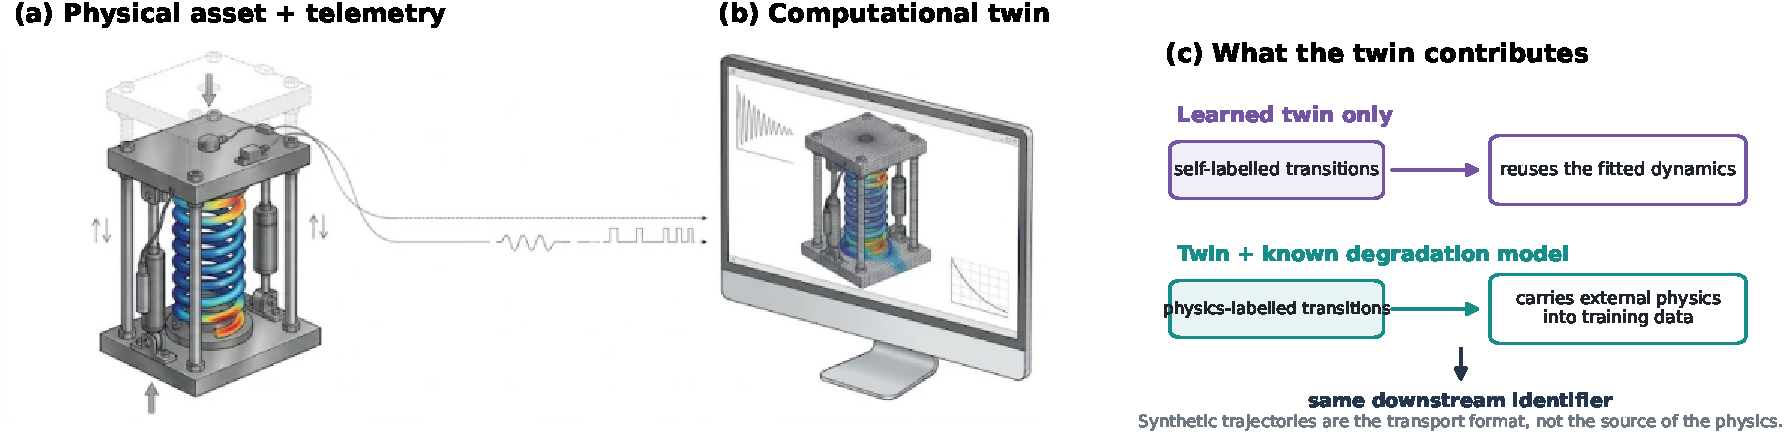
\includegraphics[width=0.95\linewidth]{figures/digital_twin_illustration.pdf}
\caption{\textbf{Illustrative digital-twin setting.} (a--b) A spring--damper asset streams telemetry to a computational counterpart; stress/deformation coloring is illustrative, not a finite-element result. (c) A learned twin produces self-labelled transitions that reuse the fitted dynamics, whereas a known component-degradation model changes those labels and transports external physics into the same training-data format.}
\label{fig:digital-twin}
\end{figure}

TRAIN has four trajectories at $w\in\{0,0.05,0.10,0.15\}$; TUNE uses $w\in\{0.025,0.125\}$. Degraded TEST uses three independent trajectories at each $w\in\{0.55,0.70,0.85\}$. The learner is ridge regression on $\phi=[x,u,wx,wu,w,1]$, with $\lambda$ selected once per seed on TUNE and then frozen for every augmentation arm. Each arm adds exactly two trajectories. The preregistered arms are duplication, recursive own-twin rollout, damping-only wrong physics, correct physics, same-regime real, and degraded real. Primary metrics are recursive degraded-TEST NRMSE at $h\in\{1,5,20\}$ and duplicate-adjusted gain.

\begin{table}[h]
\centering\small
\caption{Digital-twin paired advantage of correct degradation physics over the damping-only wrong twin. Positive values mean lower degraded-TEST NRMSE for the correct twin. Bootstrap resamples seeds.}
\label{tab:digital-twin}
\begin{tabular}{rrrr}
\toprule
$h$ & mean advantage & 95\% CI & positive seeds\\
\midrule
1  & 0.00462 & [0.00403, 0.00517] & 39/40\\
5  & 0.04122 & [0.03839, 0.04415] & 40/40\\
20 & 0.14650 & [0.13847, 0.15467] & 40/40\\
\bottomrule
\end{tabular}
\end{table}

\paragraph{Same-support self-label diagnostic.}
After the frozen study, we performed an algebraic diagnostic using exactly the high-degradation feature rows $C$ from the correct physics twin. Replacing their physical targets by the base learner's own targets, $U=C\widehat\Theta$, yields mean relative update $3.0\times10^{-15}$ (maximum $1.03\times10^{-14}$) over 40 seeds, and recursive NRMSE numerically identical to the base learner (maximum absolute difference $6.7\times10^{-9}$ at $h=20$). With the same $C$ and physical labels, the median $h=20$ improvement over the base learner is $0.762$. This diagnostic was not preregistered and is used only as a direct numerical realization of the self-consistency corollary in the main paper.

\paragraph{Long-horizon instability and secondary maintenance metric.}
Recursive high-degradation extrapolation exposes a second digital-twin failure mode. At $h=20$, NRMSE exceeds 10 in 9/40 duplicate seeds and 11/40 recursive own-twin seeds, compared with 0/40 for both physics-twin arms and degraded-real augmentation. The threshold 10 is a post-hoc descriptive instability flag, not a primary endpoint. The preregistered vibration-threshold crossing metric is mixed: the correct physics arm is not uniformly best under the fixed diagnostic excitation. We therefore do not use that secondary metric as headline evidence. The main claim is restricted to degraded-state forecasting and the exact same-support self-label control.

\subsection{Digital-twin interpretation: external information transport and finite exposure}\label{app:twin-interpretation}
This subsection gives the full interpretation behind the digital-twin section of the main paper.

\paragraph{Same support, different information.}
Let $C$ denote the fixed high-degradation feature matrix from the correct-physics arm. The base ridge solution satisfies $H\widehat\Theta=\Phi^\top Y$. If $C$ is labelled by the base twin itself, $U_{\mathrm{self}}=C\widehat\Theta$, then the augmented normal equations are
\[
(H+C^\top C)\widehat\Theta_C
=H\widehat\Theta+C^\top C\widehat\Theta
=(H+C^\top C)\widehat\Theta,
\]
so $\widehat\Theta_C=\widehat\Theta$ exactly. The numerical diagnostic (mean relative update $3.0\times10^{-15}$; maximum $1.03\times10^{-14}$) is therefore not an empirical coincidence but a direct finite-precision realization of the algebra.

Now let $A_{\mathrm{deg}}$ denote external information specifying a component degradation law. A self-generated twin samples from a kernel $K_{\mathrm{self}}(\cdot\mid D)$, whereas a physics twin samples from $K_{\mathrm{phys}}(\cdot\mid D,A_{\mathrm{deg}})$. Hence
\[
I(\theta;Z_{\mathrm{self}}\mid D)=0,
\qquad
I(\theta;Z_{\mathrm{phys}}\mid D,A_{\mathrm{deg}})=0.
\]
The second equality does \emph{not} say the physics twin is uninformative relative to $D$ alone: the additional source is $A_{\mathrm{deg}}$. The trajectory is an encoding/transport mechanism that converts this side information into examples compatible with the downstream learner. In particular, when $A_{\mathrm{deg}}$ is informative about the missing degradation regime, $(D,A_{\mathrm{deg}})$ can be strictly more informative for deployment than $D$ even though $Z_{\mathrm{phys}}$ adds nothing conditional on the pair.

\paragraph{Why a wrong twin can still help.}
For a single synthetic direction $v$, write $e=\widehat\theta-\theta_\star$, $g=\theta_g-\theta_\star$, and $Q=Q_{H_f}$. Define
\[
h=v^\top H^{-1}v,\quad s=v^\top(e-g),\quad
m=v^\top H^{-1}Qe,\quad
c=v^\top H^{-1}QH^{-1}v.
\]
Sherman--Morrison yields
\[
e_\rho=e-\frac{\rho}{1+\rho h}H^{-1}vs.
\]
Writing $\alpha=\rho/(1+\rho h)$ and expanding $e_\rho^\top Qe_\rho-e^\top Qe$ gives
\[
\Delta\mathcal R_Q(\alpha)
=-2\alpha sm+\alpha^2s^2c.
\]
The derivative at zero is $-2sm$, so $sm>0$ is exactly the local condition under which a biased generator improves deployment risk. Physical correctness is therefore sufficient neither for usefulness nor for uselessness of an imperfect source: what matters is the relationship among current learner error, generator error, learner information geometry, and deployment sensitivity. The damping-only twin can satisfy $sm>0$ even with $g\neq0$; the correct twin simply produces a more favorable deployment-weighted update in the tested regime.

\subsection{Why transport physics through synthetic data rather than impose it directly?}\label{app:greybox}
A natural grey-box objection is that if $A_{\mathrm{deg}}$ is known, one could encode it directly in a constrained estimator, PINN, structured state-space model, or symbolic library rather than generate trajectories. We agree that direct incorporation can be preferable when the downstream learner exposes the appropriate architecture or optimization interface. The digital-twin experiment is not a claim of universal statistical efficiency for synthetic transport.

The distinct advantage of the synthetic representation is \emph{interoperability}. A set of transition tuples can be consumed by heterogeneous or frozen learners without modifying their internals: tree ensembles, legacy estimators, pretrained models with only a data-adaptation interface, black-box AutoML systems, or ensembles whose members support incompatible constraint languages. Synthetic data therefore act as a model-agnostic transport layer for the side information in $A_{\mathrm{deg}}$. The choice between direct grey-box incorporation and synthetic transport is itself application-dependent and should be evaluated under matched information and compute budgets.

\paragraph{Finite optimal exposure and reversal threshold.}
Assume $sm>0$, $s\neq0$, and $c>0$. As a function of effective exposure $\alpha\in[0,h^{-1})$, the quadratic risk difference is minimized at
\[
\alpha_0=\frac{m}{sc}.
\]
After accounting for the feasible interval, $\alpha^\star=\Pi_{[0,h^{-1}]}(\alpha_0)$. If $0<\alpha^\star<h^{-1}$, the corresponding raw exposure is obtained by inverting $\alpha=\rho/(1+\rho h)$:
\[
\rho^\star=\frac{\alpha^\star}{1-h\alpha^\star}.
\]
The nonzero crossing of $\Delta\mathcal R_Q$ occurs at
\[
\alpha_{\mathrm{cross}}=\frac{2m}{sc}.
\]
If $0<\alpha_{\mathrm{cross}}<h^{-1}$, then the synthetic source helps for $0<\alpha<\alpha_{\mathrm{cross}}$ but harms once $\alpha>\alpha_{\mathrm{cross}}$. In raw exposure units,
\[
\rho_{\mathrm{cross}}=\frac{\alpha_{\mathrm{cross}}}{1-h\alpha_{\mathrm{cross}}}.
\]
If $\alpha_{\mathrm{cross}}\ge h^{-1}$, increasing exposure cannot cross into harm along this fixed direction; the gain instead saturates as $\rho\to\infty$. Thus the theory predicts three qualitatively different dose-response regimes: monotone improvement to saturation, a finite interior optimum followed by degradation, or no beneficial exposure at all.

\paragraph{Horizon dependence.}
For controlled dynamics, first-order parameter sensitivities satisfy $J_{k+1}=A_kJ_k+B_k$ and induce
\[
Q_{H_f}=\sum_{k=1}^{H_f}J_k^\top W_kJ_k.
\]
Changing $H_f$ therefore changes $m$ and $c$ even if $H$, $v$, $e$, and $g$ are fixed. Long horizons can rotate and rescale the deployment-sensitive geometry toward modes amplified by the tangent dynamics. The empirical correct-minus-wrong advantages $0.00462$, $0.04122$, and $0.14650$ at $h=1,5,20$ are consistent with this mechanism, but they do not by themselves identify the individual $J_k$ contributions.

\paragraph{Direct imposition versus mirrored data.}
For an exact diagonal involution $S$, the equivariant ridge estimator uses $\tfrac12\big(f(y)+Sf(Sy)\big)$ as its model (affine analogue in standardised coordinates), fitted per output with $\alpha$ tuned on the same balanced tuning windows as every other arm (\texttt{code/\allowbreak imposed\_\allowbreak symmetry\_\allowbreak exp.py}, \texttt{imposed\_\allowbreak lorenz.py}, \texttt{silverbox\_\allowbreak imposed.py}). Table~\ref{tab:imposed} compares it with duplication and with the exact mirror. Duplication and mirror numbers reproduce the archived results exactly for Lorenz and Silverbox; Duffing is reported in raw units, in which the reflection is exact.

\begin{table}[H]\centering\small
\caption{Direct imposition of the true symmetry versus mirrored data (median balanced recursive NRMSE; Silverbox at $h=10$). Silverbox has no false-imposition arm. Last column: seeds or records in which imposing beats mirroring.}\label{tab:imposed}
\begin{tabular}{@{}llccccc@{}}
\toprule
System & Learner & Dupl. & Mirrored & Imposed & Imposed & Imposed beats\\
 & & & & & (false $S$) & mirrored\\
\midrule
Lorenz (30) & Linear AR(4) & 0.137 & 0.106 & 0.099 & 0.154 & 27/30\\
 & Quadratic lib. & 0.072 & 0.036 & 0.016 & 0.117 & 29/30\\
Duffing (30) & Linear AR(4) & 0.050 & 0.050 & 0.051 & 0.076 & --\\
 & Cubic lib. & 0.132 & 0.030 & 0.028 & 0.178 & 27/30\\
Silverbox (10) & Linear ARX & 0.072 & 0.049 & 0.049 & -- & tie\\
 & Cubic NARX & 0.0077 & 0.0060 & 0.0059 & -- & 10/10\\
\bottomrule
\end{tabular}
\end{table}
Whenever the learner exposes the constraint, imposing a true symmetry is at least as accurate as mirroring the data, and on Lorenz with the quadratic library it is more than twice as accurate ($0.016$ versus $0.036$), even better than real data from the missing wing ($0.030$). On Duffing and Silverbox the two are within a few percent, and in the linear Duffing model the symmetry is already implied by the model class. Imposing the \emph{false} reflection is as harmful as mirroring it. Two conclusions follow. The certificate is needed either way, because both routes fail on a false symmetry. And the value of mirrored data is interoperability, not accuracy: it reaches the learner through the data interface alone, which is the case for frozen or heterogeneous learners, but a user who controls the architecture should impose a certified symmetry. The comparison covers ridge learners and diagonal symmetries; we did not impose the symmetry in the MLP.

\section{Certifying the twin's degradation law}\label{app:twin-screen}
\paragraph{Twin re-implementation.} For the studies in this section we re-implemented the protocol of Supplement~\ref{app:digital-twin} from its written specification, fixing the details it leaves open before running: $m_1$ is tied to ground by $(k_1,c_1)$ and $m_2$ by $(k_2(w),c_2(w))$, coupled by $(k_c,c_c)$; the input is a four-tone multisine plus a small PRBS. The re-implementation reproduces the frozen study's pattern: at observed wear $\le0.15$ and nominal noise, the correct law beats the damping-only law by $0.006$ at $h=1$ and $0.093$ at $h=20$ (40/40 seeds each), and duplicate-only rollouts exceed NRMSE 10 at $h=20$ in 9/40 seeds (frozen study: 9/40).

\paragraph{Two screens.} Both use the main-text gate (accept the lowest-defect candidate if $d_{(1)}\le0.5$ and $d_{(1)}/d_{(2)}\le0.5$). The \emph{black-box} screen compares the ridge learner's change in one-step map between the lowest and highest seen wear with the same change under each law in the nominal twin. The \emph{structured} screen fits the twin's own equation for mass~2 to low-pass-filtered observations, giving support stiffness and damping at each seen wear level, and compares their relative changes with each law's, weighting by inverse squared standard errors. For both, a law that predicts no change has defect exactly $1$. The binary screen applies the same gate to the two laws compared in the main study (correct versus damping-only).

\paragraph{History.} The black-box screen was declared first and run on seeds 13000--13039; it abstained in every seed and setting. The structured screen was then developed on seeds 14000--14009 (low-pass filtering proved necessary because errors-in-variables bias otherwise swamps the wear trend), frozen, and run with both screens on fresh seeds 15000--15039. Only the final run is reported.

\begin{table}[h]
\centering\small
\caption{Seeds (of 40) certifying the correct law; ``wrong'' counts accepts of any other law.}
\label{tab:twin-screen}
\setlength{\tabcolsep}{5pt}
\begin{tabular}{rrrrrrr}
\toprule
seen wear $\le$ & noise & black-box & binary: correct & binary: wrong & five-law: correct & five-law: wrong\\
\midrule
$0.05$ & $0$ & 40 & 39 & 0 & 23 & 0 \\
$0.05$ & $0.25$ & 0 & 18 & 0 & 0 & 0 \\
$0.05$ & $1$ & 0 & 0 & 0 & 0 & 0 \\
$0.05$ & $4$ & 0 & 0 & 0 & 0 & 0 \\
$0.15$ & $0$ & 40 & 40 & 0 & 37 & 0 \\
$0.15$ & $0.25$ & 0 & 39 & 0 & 3 & 1 \\
$0.15$ & $1$ & 0 & 8 & 0 & 0 & 0 \\
$0.15$ & $4$ & 0 & 0 & 0 & 0 & 0 \\
$0.30$ & $0$ & 40 & 40 & 0 & 40 & 0 \\
$0.30$ & $0.25$ & 1 & 40 & 0 & 17 & 0 \\
$0.30$ & $1$ & 0 & 29 & 0 & 0 & 0 \\
$0.30$ & $4$ & 0 & 2 & 0 & 0 & 0 \\
\bottomrule
\end{tabular}
\end{table}
The black-box learner's view of degradation is too noisy to certify anything once sensors are noisy, while the twin's own equations certify the correct law over the damping-only alternative whenever the seen wear range is wide enough relative to the noise, and never the reverse. Distinguishing the correct law from a stiffness-only law, which differs only in a damping change that is barely visible at light wear, needs much cleaner data; the single wrong five-law accept is exactly this near-miss. Damping is the weakly identified part, mirroring how the Duffing library failed on its weakly identified even terms.

\begin{table}[h]
\centering\small
\caption{Median duplicate-adjusted degraded-test gain at nominal noise.}
\label{tab:twin-screen-value}
\begin{tabular}{lrrrrrr}
\toprule
seen wear, $h$ & own twin & no law & damping-only & correct & binary-gated & degraded real\\
\midrule
$\le0.15$, $h=1$ & $-6.07$ & $+0.069$ & $+0.069$ & $+0.073$ & $0.000$ & $+0.069$\\
$\le0.15$, $h=20$ & $-81.2$ & $+0.664$ & $+0.674$ & $+0.802$ & $0.000$ & $+0.688$\\
$\le0.30$, $h=1$ & $-0.002$ & $+0.011$ & $+0.012$ & $+0.015$ & $+0.004$ & $+0.016$\\
$\le0.30$, $h=20$ & $-0.024$ & $+0.185$ & $+0.193$ & $+0.270$ & $+0.153$ & $+0.169$\\
\bottomrule
\end{tabular}
\end{table}
Every physics twin, even one with no degradation, rescues a duplicate-only learner whose wear extrapolation diverges; the correct law helps most. When the gate abstains the gated arm is the duplicate, which is why its median is zero at narrow seen wear: certification is a statement about trust, and abstaining from synthetic data costs accuracy when the uncertified twin would still have helped. With noise-free data the base learner already extrapolates in wear, and the twin's nominal-parameter mismatch makes every law slightly harmful ($h=20$ median $-0.029$ for the correct law at seen wear $\le0.15$).

\subsection{Dose--response}\label{app:exposure}
\begin{figure}[H]
\centering
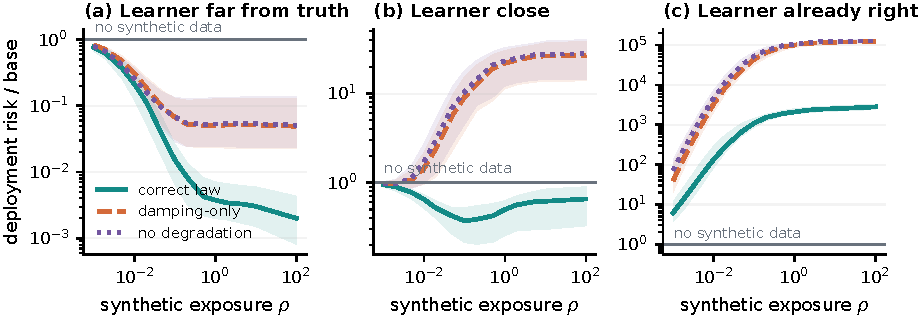
\includegraphics[width=0.88\linewidth]{figures/exposure_study.pdf}
\caption{\textbf{Dose--response: Theorem~\ref{thm:excitation}'s three regimes on the twin.} One-step deployment risk relative to the base learner as a fixed synthetic block is weighted by $\rho$ (medians, interquartile bands, 40 seeds). (a) Light wear seen, nominal noise: every law helps and saturates at its own bias. (b) Wear up to $0.30$, quarter noise: interior optimum, then harm. (c) Same, noise-free: any exposure hurts.}
\label{fig:exposure}
\end{figure}
On fresh seeds 16000--16039 we fit the base learner, build one two-trajectory block per law at wear $0.65$ and $0.85$, and refit with the block's rows weighted by $\rho\in\{0,0.001,\dots,100\}$, keeping the tuned ridge penalty fixed. One-step deployment risk is $\|\Phi_{\rm dep}(\widehat\Theta_\rho-\Theta_\star)\|^2$ on noise-free trajectories at wear $0.55$--$0.85$, with $\Theta_\star$ the least-squares map on those trajectories; this is exactly the quadratic risk $\mathcal R_Q$ of Theorem~\ref{thm:excitation}. Theorem~\ref{thm:excitation}'s closed form is for a rank-one block $G=\rho vv^\top$, whereas the experimental block has many directions; the experiment therefore tests the qualitative regimes (saturation, interior optimum, harm), not the rank-one formula itself.

\begin{table}[h]
\centering\small
\caption{Medians over 40 seeds: optimal exposure, risk at the optimum and at $\rho=100$, both relative to no synthetic data.}
\label{tab:exposure}
\setlength{\tabcolsep}{4pt}
\begin{tabular}{llrrrrrr}
\toprule
& & \multicolumn{3}{c}{one-step deployment risk} & \multicolumn{3}{c}{recursive $h=20$ error}\\
seen wear, noise & law & $\rho^\star$ & best & $\rho=100$ & $\rho^\star$ & best & $\rho=100$\\
\midrule
$\le0.15$, $1$ & correct & 100 & 0.002 & 0.002 & 100 & 0.24 & 0.24\\
 & damping-only & 0.5 & 0.048 & 0.049 & 50 & 0.36 & 0.39\\
 & none & 0.5 & 0.050 & 0.051 & 0.5 & 0.37 & 0.40\\
$\le0.30$, $0.25$ & correct & 0.1 & 0.34 & 0.65 & 0.1 & 0.81 & 0.87\\
 & damping-only & 0.002 & 0.97 & 26.7 & 0.002 & 0.99 & 3.3\\
 & none & 0.0015 & 0.96 & 27.9 & 0.001 & 0.99 & 3.5\\
$\le0.30$, $0$ & correct & 0 & 1 & 2810 & 0 & 1 & 60\\
 & damping-only & 0 & 1 & $1.2\times10^5$ & 0 & 1 & 340\\
 & none & 0 & 1 & $1.3\times10^5$ & 0 & 1 & 362\\
\bottomrule
\end{tabular}
\end{table}
The three regimes line up with the three cases of Theorem~\ref{thm:excitation}. A learner that has seen only light wear under noise is so far off at high wear that any physics source beats it in every deployment direction, so exposure helps until the learner simply copies the source, and the wrong laws stop at their own bias. A learner that has seen more wear with cleaner data is already close, so a biased source helps only in a few directions: a small dose helps, a large one imposes the source's bias. A learner that is already right ($sm\le0$ in every direction) can only be hurt. Even the correct law shows an interior optimum in the middle regime, because the twin's nominal masses and stiffnesses differ slightly from the plant's: correct mechanism, slightly wrong numbers.



\subsection{Closed-loop check: control designed on the learned model}\label{app:closedloop}
Section~\ref{sec:digital-twin} evaluates prediction. Here the learned model is used for control. For each of $40$ fresh seeds (\texttt{17000}--\texttt{17039}, same wear range and noise as the screen, \texttt{code/closed\_loop\_exp.py}), the model fitted with each arm is linearized at wear $0.7$, an infinite-horizon LQR is computed on it ($Q=\mathrm{diag}(1,1,0.1,0.1)$, $R=0.01$), and the controller is run on the \emph{true} plant at the same wear from three initial states. We report the cost relative to the LQR designed on the true plant (1 is optimal) and the number of seeds whose closed loop is unstable. The controller and cost are fixed before the run; seeds 100--107 were used only to debug the code.
\begin{table}[H]\centering\small
\caption{Closed-loop cost ratio on the true plant (median over 40 seeds) and unstable closed loops.}\label{tab:closedloop}
\begin{tabular}{lcc}
\toprule
Arm & Median cost ratio & Unstable\\
\midrule
Duplication & 1.77 & 9\\
Own-twin (learner rollout) & 1.31 & 8\\
Correct law & 1.008 & 0\\
Damping-only law & 1.007 & 0\\
Stiffness-only law & 1.007 & 0\\
No law (nominal) & 1.005 & 0\\
Overstated law & 1.024 & 0\\
Real data at the same wear (reference) & 1.070 & 0\\
Gate (abstains in 39 of 40) & 1.77 & 9\\
\bottomrule
\end{tabular}
\end{table}
Any physics-based twin, correct or not, brings the controller within $3\%$ of optimal, and duplication leaves it $77\%$ above on median with unstable loops in $9$ of $40$ seeds. Two cautions follow. First, this task does not discriminate between laws: the LQR gain depends on the linearization at one wear level, which every twin pins down roughly, so the symbolic gate is not shown to matter for control. Second, in this noisy light-wear regime the gate abstained in $39$ of $40$ seeds, so the gated arm is duplication and inherits its failures; the gate's conservatism is a cost here. Feedback also changes the excitation the learner sees, which we hold fixed. The experiment supports exposing a twin's rollouts where the control cost is sensitive; it does not show that the screening step improves control.

\section{Risk--coverage of the symbolic gate}\label{app:riskcov}
The main text fixes the absolute threshold at $\tau=0.5$ and the ratio at $0.5$. Here $\tau$ varies with the ratio fixed, on the stored per-seed defects of every screen (\texttt{code/\allowbreak gate\_\allowbreak riskcov.py}; no new simulation). Each setting's seeds are the unit; settings are not pooled into one rate.
\begin{table}[H]\centering\small
\caption{Acceptances and wrong acceptances (out of the seeds in each setting) at the threshold used and at three times it, with the Wilson 95\% upper bound on the wrong-acceptance rate.}\label{tab:riskcov}
\begin{tabular}{@{}lccccc@{}}
\toprule
 & \multicolumn{2}{c}{$\tau=0.5$ (used)} & \multicolumn{2}{c}{$\tau=1.5$} & Wrong rate,\\
\cmidrule(lr){2-3}\cmidrule(lr){4-5}
Setting (seeds) & accept & wrong & accept & wrong & upper 95\%\\
\midrule
Lorenz (exact symmetry) (30) & 17 & 0 & 23 & 0 & 0.11\\
Lorenz, broken by 2 (approx.) (20) & 13 & 0 & 17 & 0 & 0.16\\
Lorenz, broken by 5 (approx.) (20) & 8 & 0 & 15 & 0 & 0.16\\
Lorenz, broken by 10 (approx.) (20) & 9 & 0 & 15 & 0 & 0.16\\
Duffing, noise-free (30) & 29 & 0 & 30 & 0 & 0.11\\
Duffing, 1/4 noise (30) & 0 & 0 & 0 & 0 & 0.11\\
Duffing, 1/2 noise (30) & 0 & 0 & 0 & 0 & 0.11\\
Duffing, nominal noise (30) & 0 & 0 & 0 & 0 & 0.11\\
Lotka--Volterra (no symmetry) (30) & 0 & 0 & 0 & 0 & 0.11\\
Twin, wear $\le$0.05, noise $\times$0 (40) & 23 & 0 & 23 & 0 & 0.09\\
Twin, wear $\le$0.05, noise $\times$0.25 (40) & 0 & 0 & 0 & 0 & 0.09\\
Twin, wear $\le$0.05, noise $\times$1 (40) & 0 & 0 & 0 & 0 & 0.09\\
Twin, wear $\le$0.05, noise $\times$4 (40) & 0 & 0 & 0 & 0 & 0.09\\
Twin, wear $\le$0.15, noise $\times$0 (40) & 37 & 0 & 37 & 0 & 0.09\\
Twin, wear $\le$0.15, noise $\times$0.25 (40) & 4 & 1 & 4 & 1 & 0.13\\
Twin, wear $\le$0.15, noise $\times$1 (40) & 0 & 0 & 0 & 0 & 0.09\\
Twin, wear $\le$0.15, noise $\times$4 (40) & 0 & 0 & 0 & 0 & 0.09\\
Twin, wear $\le$0.3, noise $\times$0 (40) & 40 & 0 & 40 & 0 & 0.09\\
Twin, wear $\le$0.3, noise $\times$0.25 (40) & 17 & 0 & 17 & 0 & 0.09\\
Twin, wear $\le$0.3, noise $\times$1 (40) & 0 & 0 & 0 & 0 & 0.09\\
Twin, wear $\le$0.3, noise $\times$4 (40) & 0 & 0 & 0 & 0 & 0.09\\
\bottomrule
\end{tabular}
\end{table}
Two features matter. The symmetry screens are not knife-edge: no wrong acceptance occurs below $\tau=2$, and between $0.5$ and $1.5$ coverage grows where the true symmetry is present (Lorenz from 17 to 23 of 30; the broken-symmetry Lorenz settings, whose exact reflection is only approximately true, likewise). The twin's one wrong acceptance (wear seen up to $0.15$, quarter noise) appears at every threshold from $0.2$ upward, because there the wrong law's defect is as low as the correct one's; only the ratio rule or more data could exclude it. Zero observed wrong acceptances in a setting of 30 seeds still allows a true rate of up to about $0.11$. Conditional on acceptance the picture differs: the symmetry screens made 46 acceptances with none wrong, the twin screens 121 with one wrong, and that one is among only four acceptances in its setting, so the pooled rate of 1 in 660 decisions (1 in 167 acceptances) understates the risk in the hardest case.

\section{Synthetic rows and calibrated uncertainty}\label{app:coverage}
\paragraph{Scope.} The intervals below are those of a naive pipeline that counts every weighted synthetic row as an independent observation. A Bayesian model that represents the dependence of synthetic rows on the data would not shrink its intervals this way; the experiment measures what the naive pipeline loses and which simple repair recovers it.

\paragraph{Protocol.} For 40 fresh seeds (\texttt{18000}--\texttt{18039}; \texttt{code/\allowbreak coverage\_\allowbreak exp.py}) the twin's learner, alpha and synthetic blocks are built exactly as in the screening study. Each synthetic block is weighted by an exposure $\rho\in\{0,0.25,\dots,8\}$, the ridge posterior is computed treating every weighted row as an observation, and the 90\% one-step predictive interval $\hat y\pm1.645\,\hat\sigma\sqrt{1+z^\top H^{-1}z}$ is scored on the nine deployment trajectories (wear $0.55$--$0.85$) and on four fresh trajectories at the training wear levels. The noise variance $\hat\sigma^2$ is estimated either from all weighted rows (the naive pipeline) or from the real rows only. Arms: duplication, self-labels (the learner's one-step predictions on the correct-law states), the correct, damping-only and no-degradation laws, and fresh plant data at the same high-wear inputs.
\begin{table}[H]\centering\small
\caption{Median coverage of nominal 90\% intervals at exposure $\rho=8$ ($\rho=0$: $0.89$ seen, $0.87$ deployment), and median one-step error (RMSE in units of the state scale) in the seen regime.}\label{tab:coverage}
\begin{tabular}{@{}lccccc@{}}
\toprule
 & \multicolumn{2}{c}{Noise from all rows} & \multicolumn{2}{c}{Noise from real rows} & Error\\
\cmidrule(lr){2-3}\cmidrule(lr){4-5}
Arm & seen & deployment & seen & deployment & seen\\
\midrule
Duplication & 0.89 & 0.68 & 0.89 & 0.69 & 0.153\\
Self-labels & 0.53 & 0.39 & 0.89 & 0.74 & 0.151\\
Correct law & 0.54 & 0.54 & 0.90 & 0.90 & 0.147\\
Damping-only law & 0.54 & 0.51 & 0.90 & 0.88 & 0.148\\
No-degradation law & 0.54 & 0.51 & 0.90 & 0.88 & 0.147\\
Fresh real data & 0.89 & 0.89 & 0.90 & 0.90 & 0.148\\
\bottomrule
\end{tabular}
\end{table}
\paragraph{Proof of Proposition~\ref{prop:overconf}.} Weighted ridge with self-labelled rows solves $(H+\rho C^\top C)\theta=\Phi^\top Y+\rho C^\top C\widehat\theta$, and $\theta=\widehat\theta$ satisfies it because $H\widehat\theta=\Phi^\top Y$; so the estimate and every real residual are unchanged, and every synthetic residual is $C\widehat\theta-C\widehat\theta=0$. The naive variance estimate divides the unchanged weighted residual sum by $n+\rho m-p$ instead of $n-p$, so $\widehat\sigma_\rho^2=k\,\widehat\sigma_0^2$. The naive predictive variance at $x$ is $\widehat\sigma_\rho^2(1+\ell_\rho(x))$, so the half-width is the base half-width times $\sqrt{k(1+\ell_\rho(x))/(1+\ell_0(x))}$. For (a), the error at a fresh point is $\epsilon+x^\top(\theta_\star-\widehat\theta)$ with $\epsilon\sim\mathcal N(0,\sigma^2)$; as $n\to\infty$ with $\rho m/n$ fixed, $x^\top(\theta_\star-\widehat\theta)\to0$, $\ell_\rho,\ell_0\to0$ and $\widehat\sigma_0\to\sigma$, so the interval $\pm z_{\alpha/2}\widehat\sigma_\rho\sqrt{1+\ell_\rho}$ covers with probability tending to $P(|\epsilon|\le z_{\alpha/2}\sigma\sqrt k)=2\Phi(z_{\alpha/2}\sqrt k)-1$. For (b), with $\widehat\sigma^2$ from the real rows the first factor is $1$ and only $(1+\ell_\rho)/(1+\ell_0)\le1$ remains; it is near $1$ where $\ell_0(x)$ is small (well-observed inputs) and can be small where $\ell_0(x)$ is large, which is where the synthetic rows were placed. \hfill$\blacksquare$

\textbf{Intuition:} the pipeline books every synthetic row as a measurement that fitted perfectly, so it believes the system is quieter than it is, by exactly the share of rows that are synthetic. Taking the noise from real rows removes that error, but the synthetic rows still claim to have pinned down the parameters in the very region nobody observed.

\begin{table}[H]\centering\small
\caption{Coverage predicted by Proposition~\ref{prop:overconf}(a) ($n=1196$, $m=598$, $p=12$, nominal $z$, no fitted constant) and observed medians, seen regime.}\label{tab:overconf}
\begin{tabular}{@{}lccccccc@{}}
\toprule
Exposure $\rho$ & 0 & 0.25 & 0.5 & 1 & 2 & 4 & 8\\
\midrule
Predicted & 0.900 & 0.879 & 0.858 & 0.820 & 0.754 & 0.656 & 0.536\\
Self-labels & 0.894 & 0.870 & 0.849 & 0.811 & 0.743 & 0.648 & 0.530\\
Correct law & 0.894 & 0.878 & 0.858 & 0.818 & 0.753 & 0.657 & 0.539\\
\bottomrule
\end{tabular}
\end{table}

Three mechanisms are visible. Self-labels leave every prediction unchanged (largest change $7\times10^{-14}$, the self-consistency limit) yet tighten the intervals, through a smaller noise estimate in the seen regime and through a smaller parameter-uncertainty term in the unseen one; only the first is undone by estimating noise from real rows. Noiseless law-based rows deflate the noise estimate whether or not the law is right; with noise estimated from real rows, all three laws are calibrated at one step, because their one-step bias is small (the multi-step consequences of a wrong law are in Section~\ref{sec:digital-twin}). Duplication barely changes coverage in the seen regime, where intervals are dominated by noise, but loses coverage at deployment because reweighting the two highest-wear training trajectories moves the fit. Fresh real data hold nominal coverage throughout. The practical rule is in Table~\ref{tab:regimes}: never estimate noise from synthetic rows, and never let self-generated rows shrink uncertainty about a regime that was not observed.

\section{Digital twins in practice: a Bayesian and learning-for-dynamics reading}\label{app:bayes-twins}
This section places the results next to current twin practice. It is a framing, not a survey: we cite only what we use, and the simulations below are linear-Gaussian illustrations, not evidence about any particular twin.

\subsection{A synthetic block is a prior}
Take the ridge learner of Theorem~\ref{thm:excitation} as the posterior mean of a Gaussian linear model with noise variance $\sigma^2$. A noiseless synthetic block with regressors $\Phi_g$, generator parameter $\theta_g$ and exposure $\rho$ moves the estimate exactly as a Gaussian prior $\theta\sim\mathcal N\big(\theta_g,\ \sigma^2\rho^{-1}(\Phi_g^\top\Phi_g)^{-1}\big)$ would, since $e_G=(H+G)^{-1}(He+Gg)$ is the posterior-mean formula with prior mean $\theta_g$ and prior precision $G$ (a \emph{power prior} in the sense of \citealp{ibrahim2000power}, with $\rho$ the power). Three consequences follow, and each is a Bayesian restatement of a result in the paper.
\begin{itemize}[leftmargin=1.2em,itemsep=1pt,topsep=2pt]
\item \emph{Closure.} Rollouts of the fitted model have $\theta_g=\widehat\theta$, so the posterior mean does not move (the self-consistency limit), while the posterior covariance shrinks from $\sigma^2H^{-1}$ to $\sigma^2(H+G)^{-1}$. Treating self-generated trajectories as evidence therefore changes no point estimate and manufactures certainty.
\item \emph{Finite optimum.} Theorem~\ref{thm:excitation} is the bias--variance trade of an informative prior with a wrong mean: the prior pulls toward $\theta_g$ (bias $\propto s$, the generator's error along $v$) and removes variance (excitation, $h$). The best exposure $\alpha^\star=\Pi_{[0,h^{-1}]}(m/(sc))$ is the best prior strength for a given misspecification.
\item \emph{Dose from data.} The exposure $\rho$ is a hyperparameter, so it can be chosen by marginal likelihood (empirical Bayes) or a held-out loss instead of being fixed at one.
\end{itemize}

\paragraph{Numerical check (\texttt{code/bayes\_view.py}).} A linear-Gaussian problem with $d=8$ parameters, $n=20$ real rows, $m=40$ synthetic rows and $\sigma=0.5$ (600 draws per row of Table~\ref{tab:bayes}). The identity above holds to machine precision. ``Self'' uses rollouts of the fitted model with exposure $1$; ``twin'' uses a generator with parameter error of the stated size; ``EB'' chooses $\rho$ on a grid by marginal likelihood. Coverage is that of nominal $90\%$ credible intervals for the response at fresh inputs.
\begin{table}[H]\centering\small
\caption{Bayesian reading of a synthetic block: median parameter-prediction error and mean coverage of nominal 90\% intervals.}\label{tab:bayes}
\begin{tabular}{@{}lcccccc@{}}
\toprule
 & \multicolumn{3}{c}{Prediction error} & \multicolumn{3}{c}{Coverage of 90\% intervals}\\
\cmidrule(lr){2-4}\cmidrule(lr){5-7}
Twin bias & real only & $\rho{=}1$ & EB & real & self & EB\\
\midrule
0 (exact) & 0.144 & 0.004 & 0.000 & 0.91 & 0.46 & 0.99\\
0.3 & 0.147 & 0.056 & 0.058 & 0.90 & 0.45 & 0.68\\
1 & 0.140 & 0.590 & 0.123 & 0.91 & 0.45 & 0.87\\
3 & 0.144 & 5.396 & 0.178 & 0.90 & 0.45 & 0.84\\
\bottomrule
\end{tabular}
\end{table}
Treating rollouts of the fitted model as evidence halves the coverage of nominal $90\%$ intervals without changing the estimate. A biased twin at fixed exposure $1$ is far worse than no twin once the bias is moderate ($0.59$ versus $0.14$), while choosing the exposure by marginal likelihood recovers most of the oracle's accuracy ($0.12$ versus $0.10$ at bias $1$). It is not a cure: at the largest bias it is slightly worse than using no twin ($0.178$ versus $0.144$, because the grid's smallest exposure is $0.01$ rather than $0$), and its intervals are still too narrow when the bias is small to moderate (coverage $0.68$ at bias $0.3$). Calibrated twins need the mismatch itself to be modelled, not only its dose.

\subsection{How this sits next to twin practice}
Current twin work uses several tools, and the results above say which job each does.
\begin{itemize}[leftmargin=1.2em,itemsep=1pt,topsep=2pt]
\item \emph{Bayesian parameter updating and data assimilation} (for example probabilistic graphical-model twins, \citealp{kapteyn2021probabilistic}) fold real measurements into the twin's own parameters. This is the right tool when the twin's structure is trusted and the consumer of the twin is that parametric model; nothing here contradicts it, and information closure is its own consistency condition. We study a different case: a \emph{separate} learner, possibly frozen or of another model class, that can only receive information as data.
\item \emph{Grey-box and physics-informed learning} \citep{raissi2019pinn} imposes structure on the learner. Table~\ref{tab:imposed} shows that, when a learner exposes the constraint, imposing a certified symmetry is at least as accurate as mirrored data; synthetic transport earns its place through interoperability, not accuracy.
\item \emph{Synthetic data for maintenance} \citep{nieminen2026synthetic,wuttke2026digital} generates labelled data from simulation. Our claim about this practice is narrow: such data add information only to the extent that the simulator's law is right (provenance); a biased law can have an interior best dose under specified alignment conditions (Theorem~\ref{thm:excitation}); and the law can be screened from the seen data, imperfectly (Proposition~\ref{prop:sandwich}). In our simulated twin a correct law improved median $h=20$ error by $0.762$ and cut closed-loop cost excess from $77\%$ to under $3\%$, so the practice works when its premise holds.
\end{itemize}
A workable protocol follows: (i) state which generator produced each block and whether it carries external structure; (ii) screen candidate laws against the seen data and abstain when no candidate stands out; (iii) set the dose by held-out loss or marginal likelihood, never by availability; (iv) always compare with duplication and, where possible, with direct imposition; (v) for control, direct exposure at the directions where the closed-loop cost is sensitive, which is the role of $Q$ in Theorem~\ref{thm:excitation}.

\subsection{A learning-for-dynamics view}
Persistent excitation says which \emph{real} experiments identify a system; Theorem~\ref{thm:excitation} is its synthetic counterpart and says which \emph{simulated} experiments help, with the added possibility that the experiment is biased and so harmful past a finite dose. The gate is a certificate in the sense of safe learning: a structure is used only when the seen data already support it, and the sandwich bound says when that is possible. Four limits bound the claims: the theory is for ridge learners; Proposition~\ref{prop:finite} assumes an exogenous design, so a recursive-dynamics version needs an errors-in-variables term; the maintenance evidence is a simulated twin with one device per real benchmark; and in the closed-loop check every physics twin helped, so the gate was not shown to matter for control. Natural next steps are a calibrated Bayesian treatment that models the twin's mismatch (a hierarchical prior over $\theta_g-\theta_\star$), and closed-loop tasks whose cost, unlike an LQR at one operating point, is sensitive to the law.

\section{Broader implication: a Synthetic Information Profile}\label{app:evaluation-profile}

\paragraph{Scope relative to the main paper.}
The evaluation profile below is a broader research implication, not an additional L4DC theorem claim. In particular, MATCH$-$REAL is a content-effect control rather than a direct measurement of Shannon information, and DAL is a local empirical analogue of deployment alignment rather than the scalar $m$ in the deployment-weighted excitation theorem in the main paper outside the corresponding local model. This distinction prevents the information-theoretic and finite-learner notions from being conflated.
The theory suggests a distinction that is useful beyond the present systems. Fidelity, diversity, and privacy can be properties of a generator or generated distribution, but \emph{downstream utility is relational}. A meaningful utility statement is indexed at least by
\[
(\text{generator},\ \text{learner},\ \text{deployment task/horizon},\ \text{authentic-data regime},\ \text{synthetic budget}),
\]
plus the provenance of any external information used by the generator. This section records a concrete evaluation profile for future synthetic-time-series benchmarks; it is not needed for the main L4DC claims.

\subsection{Factorial controls: separate content from exposure}
For pretrained adaptation, use four arms with matched optimizer budgets whenever possible:
\begin{center}
\begin{tabular}{lll}
\toprule
Arm & target content & target weight/exposure\\
\midrule
REAL & authentic only & baseline\\
COPY & authentic repeated & increased\\
MATCH & real/synthetic mixture & baseline\\
AUGMENT & real + synthetic & increased\\
\bottomrule
\end{tabular}
\end{center}
Then $\mathrm{COPY}-\mathrm{REAL}$ isolates reweighting/optimization effects, while $\mathrm{MATCH}-\mathrm{REAL}$ isolates the effect of replacing authentic content with synthetic content at matched target weight. Importantly, a positive MATCH effect is not synonymous with new Shannon information: an information-closed generator can still alter a restricted learner through regularization, smoothing, representation, or misspecification. Conversely, a pretrained or physics-based generator can be information-open relative to the target block because it imports external information.

\subsection{Learner-relative metric chain}
For lower-is-better loss $L$, the following diagnostics separate different stages of synthetic value.

\paragraph{Learner-residual novelty (LRN).}
For synthetic transition rows $(C,U)$ and pre-augmentation predictor $\widehat f$,
\[
\mathrm{LRN}=\frac{\mathrm{RMS}[U-\widehat f(C)]}{\text{authentic residual or target scale}}.
\]
Near-zero LRN indicates self-consistency for the chosen learner; large LRN means only potential novelty, not quality.

\paragraph{Learner-update magnitude (LUM).}
\[
\mathrm{LUM}=\frac{\|\theta_{\mathrm{SYNTH}}-\theta_{\mathrm{DUP}}\|_H}
{\|\theta_{\mathrm{DUP}}\|_H+\varepsilon}.
\]
This asks whether the synthetic block actually moves the learner beyond matched re-exposure. It is unsigned: a large update can be harmful.

\paragraph{Deployment alignment (DAL).}
For differentiable deployment loss, define the local cosine
\[
\mathrm{DAL}=-\frac{\langle\nabla L_{\mathrm{deploy}},\Delta_{\mathrm{SYNTH}}-\Delta_{\mathrm{DUP}}\rangle}
{\|\nabla L_{\mathrm{deploy}}\|\,\|\Delta_{\mathrm{SYNTH}}-\Delta_{\mathrm{DUP}}\|}.
\]
DAL is a first-order empirical analogue of deployment alignment in the deployment-weighted excitation theorem in the main paper; it should not be described as literally equal to $m$ outside the local model.

\paragraph{Duplicate-adjusted utility (DAU).}
\[
\mathrm{DAU}=L(\mathrm{DUPLICATE})-L(\mathrm{SYNTHETIC}),
\]
with equal data exposure and training budget. DAU is the realized downstream effect, not a decomposition into $s,m,c$.

\paragraph{Real-data equivalent recovery (RER).}
When an equal-budget fresh-real arm has positive headroom,
\[
\mathrm{RER}=\frac{L(\mathrm{DUPLICATE})-L(\mathrm{SYNTHETIC})}
{L(\mathrm{DUPLICATE})-L(\mathrm{FRESH\ REAL})}.
\]
RER=0 means no value beyond re-exposure; RER=1 matches the chosen fresh-real positive control. The ratio should be suppressed when the denominator is negligible.

\paragraph{Horizon utility profile (HUP).}
\[
\mathrm{HUP}(h)=L_h(\mathrm{DUPLICATE})-L_h(\mathrm{SYNTHETIC}).
\]
Time-series utility should be displayed as a horizon curve rather than collapsed to one-step quality when recursive deployment matters.

\paragraph{Cross-learner utility profile (CLUP).}
Evaluate the same synthetic block across a fixed suite (for example linear AR, boosted/tree model, small neural forecaster, and a foundation-model adaptation head). Disagreement is scientifically meaningful because learner-relative utility is not expected to be universal.

The intended diagnostic chain is
\[
\boxed{\mathrm{LRN}\ \longrightarrow\ \mathrm{LUM}\ \longrightarrow\ \mathrm{DAL}\ \longrightarrow\ \mathrm{DAU}},
\]
interpreted as: does the block assert something new to this learner; does the learner move; is the movement locally aligned with deployment improvement; and does the improvement actually materialize? These are complementary, not interchangeable, statistics.

\subsection{Information provenance}
Every generator should carry a provenance label describing what can enter beyond the authentic training block:
\begin{itemize}
\item \textsc{Self-closed}: only authentic training data and outputs derived from them;
\item \textsc{Prior-open}: an externally pretrained model or prior;
\item \textsc{Physics-open}: equations, simulator, symmetry, constraints, or degradation law;
\item \textsc{Environment-open}: fresh interaction, reward, verifier, or external measurement;
\item \textsc{Human-open}: expert rules, labels, or feedback.
\end{itemize}
Information Closure says that a \textsc{Self-closed} generator cannot create new physical information about $\theta$ conditional on its authentic source. The other labels do not guarantee utility; they identify where genuinely external information \emph{could} have entered.

\subsection{Why this is not a universal quality score}
A synthetic series may have high marginal/spectral fidelity and low downstream value, or low pointwise resemblance and high task value. Therefore conventional fidelity diagnostics---marginals, ACF/PACF, spectra, cross-channel dependence, discriminator tests, embedding precision/recall, privacy/memorization---should remain visible but separate from learner-relative utility. The proposed profile is explicitly multidimensional rather than a weighted scalar leaderboard.

\end{document}
